\chapter{Détermination des paramètres du modèle et analyse des résultats}
\label{chap:dedetermination_des_parametres_et_analyse_des_resultats}


\section{Choix des données historiques}

Dans un GSE monde réel, le calibrage des modèles repose entièrement sur les séries historiques fournies en entrée : ce sont elles qui déterminent les paramètres de retour à la moyenne, les niveaux de long terme et les volatilités estimés. Le choix des données est donc une étape structurante, qui conditionne à la fois la qualité du calibrage et la plausibilité des scénarios projetés. Les critères retenus pour la sélection sont la cohérence géographique avec le périmètre de l'assureur modélisé (zone France / Eurozone), la disponibilité d'historiques suffisamment longs pour estimer des paramètres de long terme, et la pertinence de chaque série par rapport au modèle qui en fait usage dans le GSE.

L'ensemble des données couvre la période allant de 2004 à 2025, à pas de temps mensuel. Cette fenêtre temporelle constitue la plage la plus large rendue disponible par la conjonction des différentes sources mobilisées. Elle présente l'avantage d'englober plusieurs régimes de taux contrastés : une période de taux modérés avant la crise financière de 2008, une longue phase de taux bas et négatifs en zone euro de 2015 à 2021, puis un cycle de remontée rapide des taux amorcé en 2022. Cette diversité de régimes est précieuse pour l'estimation des paramètres d'un modèle de Vasicek, dont la robustesse dépend de la capacité des données à couvrir plusieurs cycles autour du niveau d'équilibre de long terme.

Les séries historiques retenues pour le calibrage et les projections du GSE sont les suivantes :
\begin{itemize}
    \item \textbf{Les taux d'intérêt :} \\[0.3em]
    Trois points de la courbe des taux souverains français ont été retenus : le taux 1 an, le taux 10 ans et le taux 30 ans. Ces trois taux sont issus du site "investing.com". Ces trois maturités correspondent directement aux variables modélisées dans le GSE : le taux 10 ans sert de taux long $l_t$, le taux 1 an permet de reconstituer le spread $s_t = l_t - r_t$ qui, soustrait au taux long, donne le taux court, et le taux 30 ans constitue le point d'ancrage de très long terme de la courbe des taux zéro-coupon projetée. Le recours aux taux souverains français est cohérent avec la nature du portefeuille obligataire modélisé, composé principalement d'obligations d'État françaises.
    \item \textbf{L'inflation :} \\[0.3em]
    L'inflation retenue est l'inflation française mesurée par l'indice des prix à la consommation (IPC), publiée par l'INSEE. Elle est modélisée dans le GSE par un processus d'Ornstein-Uhlenbeck, dont les paramètres sont estimés sur cette série. La période 2004-2025 est particulièrement riche pour ce calibrage, car elle couvre aussi bien les années de faible inflation proche de zéro (2014-2021) que le pic inflationniste post-Covid de 2022-2023, offrant ainsi une bonne représentation de la dispersion historique de cette variable.
    \item \textbf{Les actions :} \\[0.3em]
    L'indice retenu pour la composante actions est le STOXX Europe 600 Net Return, issu de Bloomberg. Il s'agit d'un indice large représentant les 600 plus grandes capitalisations européennes, calculé en performance totale nette (dividendes réinvestis nets de retenue à la source). Le réinvestissement des dividendes directement intégré dans les données a son importance pour mesurer le rendement global de l'investissement car le modèle ALM ne gère pas le réinvestissement des dividendes. Son utilisation est cohérente avec un portefeuille d'un assureur européen exposé aux marchés actions de la zone. Dans le GSE, cet indice alimente le mouvement brownien géométrique modélisant les actions, dont la dérive et la volatilité sont estimées à partir des log-rendements annuels observés sur la période.
    \item \textbf{L'immobilier :} \\[0.3em]
    La composante immobilière est représentée par l'indice IEIF Eurozone en valeur brute (loyers inclus), publié par l'Institut de l'Épargne Immobilière et Foncière (IEIF). Cet indice mesure la performance totale de l'immobilier d'investissement coté en zone euro et constitue le proxy de référence pour cette classe d'actifs dans les modèles d'assurance vie. Comme pour les actions, les revenus locatifs sont intégrés dans les données pour simplification du refinancement et il est utilisé pour calibrer un mouvement brownien géométrique dans le GSE. Sa valorisation annuelle alimente directement la poche immobilier du portefeuille ALM.
\end{itemize}


\section{Scénario témoin calibré par moindres carrés ordinaires}

La mise en œuvre du GSE monde réel requiert de fixer, pour chacune des variables modélisées, les paramètres qui gouvernent leur dynamique stochastique. Deux scénarios témoins sont construits à cet effet. Le premier repose sur un calibrage purement statistique, obtenu par estimation des paramètres à partir des séries historiques présentées en section~3.1, à l'aide de la méthode des moindres carrés ordinaires (MCO). Le second s'en écarte volontairement : plutôt que de refléter la moyenne des observations passées, il fixe certains paramètres à dire d'expert, de manière à représenter un environnement de taux cohérent avec les objectifs de politique monétaire affichés par la Banque Centrale Européenne. La comparaison de ces deux scénarios témoins permet d'apprécier dans quelle mesure un calibrage purement historique peut diverger d'une trajectoire jugée cohérente avec le cadre macroéconomique actuel. C'est à partir de ces deux paramétrages de référence que le chapitre suivant construira des scénarios choqués, en faisant varier volatilités, niveaux de long terme et vitesses de retour à la moyenne.

\subsection{Calibrage des paramètres par moindres carrés ordinaires}

\subsubsection{Estimation des paramètres des processus de Vasicek et d'Ornstein-Uhlenbeck}

Pour les variables modélisées par un processus de Vasicek ou d'Ornstein-Uhlenbeck — taux long, spread de taux, taux très long et inflation —, l'estimation repose sur la forme discrétisée du processus. En posant un pas de temps $\Delta t = 1$ an, la solution exacte de l'équation différentielle stochastique implique que le processus suit une régression autorégressive d'ordre 1 :
\begin{equation}
    X_{t+1} = a + b \, X_t + \varepsilon_t, \qquad \varepsilon_t \sim \mathcal{N}(0, s^2)
\end{equation}
Cette équation est estimée par MCO sur la série historique de chaque variable, ce qui fournit les coefficients $\hat{a}$, $\hat{b}$ et $\hat{s}$. Les paramètres du processus continu sont ensuite récupérés par les relations suivantes :
\begin{equation}
    \hat{\kappa} = -\ln(\hat{b}), \qquad
    \hat{\theta} = \frac{\hat{a}}{1 - \hat{b}}, \qquad
    \hat{\sigma} = \hat{s} \sqrt{\frac{2\hat{\kappa}}{1 - e^{-2\hat{\kappa}}}}
\end{equation}
où $\hat{\kappa}$ est la vitesse de retour à la moyenne, $\hat{\theta}$ le niveau de long terme et $\hat{\sigma}$ la volatilité instantanée.

\subsubsection{Estimation des paramètres des mouvements browniens géométriques}

Pour les variables modélisées par un mouvement brownien géométrique — actions et immobilier —, l'estimation repose sur les log-rendements annuels observés. Si $S_t$ désigne la valeur de l'indice à la date $t$, le log-rendement est défini par $y_t = \ln(S_t / S_{t-1})$. Sous l'hypothèse d'un mouvement brownien géométrique, ces log-rendements sont i.i.d. selon une loi normale de moyenne $\mu - \sigma^2/2$ et d'écart type $\sigma$. La dérive $\mu$ et la volatilité $\sigma$ sont estimées par :
\begin{equation}
    \hat{\sigma} = \text{std}(y_t), \qquad \hat{\mu} = \bar{y} + \frac{\hat{\sigma}^2}{2}
\end{equation}

\subsubsection{Matrice de corrélation}

Les corrélations entre variables sont estimées à partir des résidus $\hat{\varepsilon}_t$ de chacun des modèles après calibrage. Pour les processus de Vasicek, les résidus sont les termes d'erreur de la régression AR(1) ; pour les mouvements browniens géométriques, ce sont les log-rendements recentrés. La matrice de corrélation empirique est calculée sur ces résidus et rendue définie positive avant d'être utilisée pour générer des chocs corrélés dans la simulation Monte-Carlo.


\subsubsection{Paramètres estimés}

Le tableau~\ref{tab:parametres_gse_MCO} regroupe l'ensemble des paramètres estimés par MCO sur la période 2004-2025.

\begin{table}[H]
\centering
\caption{Paramètres du GSE monde réel estimés par MCO (2004–2025)}
\label{tab:parametres_gse_MCO}
\begin{tabular}{llccc}
\hline
\textbf{Variable} & \textbf{Modèle} & $\hat{\kappa}$ \textit{ou} $\hat{\mu}$ & $\hat{\theta}$ & $\hat{\sigma}$ \\
\hline
Taux 10 ans (France)   & Vasicek & 0,146 & 0,0202 & 0,00737 \\
Spread 1/10 ans   & Vasicek & 0,336 & 0,0107 & 0,006986 \\
Taux 30 ans (France)   & Vasicek & 0,176 & 0,0279 & 0,00737 \\
Inflation (France)     & Ornstein-Uhlenbeck & 0,198 & 0,0223 & 0,0123 \\
Actions (STOXX 600 NR) & GBM & 0,0776 & — & 0,139 \\
Immobilier (IEIF EZ)   & GBM & 0,0657 & — & 0,200 \\
\hline
\end{tabular}
\end{table}


Les trois points de la courbe des taux souverains français présentent des vitesses de retour à la moyenne $\hat{\kappa}$ nettement différenciées. Le spread 1 an / 10 ans revient le plus rapidement vers son niveau d'équilibre, avec $\hat{\kappa} = 0{,}336$, soit une demi-vie $\ln(2)/\hat{\kappa}$ d'environ deux ans. La demi-vie étant le temps nécessaire pour que la variable parcours la moitié de la distance qui la sépare de sa valeur moyenne de long terme. L'écart entre taux court et taux long se résorbe donc relativement vite, ce qui traduit la sensibilité de la partie courte de la courbe aux décisions de politique monétaire. À l'inverse, le taux 10 ans ($\hat{\kappa} = 0{,}146$) et le taux 30 ans ($\hat{\kappa} = 0{,}176$) affichent des demi-vies plus longues, respectivement proches de 4{,}7 et 3{,}9 ans, cohérentes avec l'inertie usuellement observée sur les segments longs de la courbe des taux.

Les niveaux de long terme estimés dessinent une structure par terme croissante et économiquement cohérente : $\hat{\theta}$ vaut 2{,}02\,\% pour le taux 10 ans et 2{,}79\,\% pour le taux 30 ans, soit une pente positive d'environ 77 points de base entre ces deux maturités à l'équilibre. Le niveau de long terme du taux court peut être retrouvé par différence entre le taux long et le spread, soit $\hat{\theta}_{10y} - \hat{\theta}_{spread} = 2{,}02\,\% - 1{,}07\,\% = 0{,}95\,\%$ : le modèle projette ainsi, à très long terme, une courbe des taux nettement pentue, avec un taux court proche de 1\,\% et un taux 30 ans proche de 2{,}8\,\%. Les volatilités instantanées $\hat{\sigma}$ du taux 10 ans et du taux 30 ans sont identiques (0{,}737\,\%), tandis que celle du spread est légèrement inférieure (0{,}699\,\%), ce qui reflète la corrélation élevée entre les mouvements des différents points de la courbe.

L'inflation française est estimée avec une vitesse de retour à la moyenne $\hat{\kappa} = 0{,}198$, proche de celle des taux longs, correspondant à une demi-vie d'environ 3{,}5 ans. Son niveau de long terme, $\hat{\theta} = 2{,}23\,\%$, est très proche de la cible de 2\,\% visée par la Banque Centrale Européenne, ce qui constitue un point de cohérence notable entre le calibrage purement statistique et l'objectif affiché de politique monétaire. Sa volatilité ($\hat{\sigma} = 1{,}23\,\%$) est en revanche sensiblement supérieure à celle des taux d'intérêt, ce qui s'explique par l'amplitude des variations d'inflation observées sur la période 2004-2025, et en particulier par l'épisode inflationniste de 2022/2023.

Pour les actions et l'immobilier, modélisés par un mouvement brownien géométrique, les paramètres estimés sont la dérive annuelle $\hat{\mu}$ et la volatilité annuelle $\hat{\sigma}$ des log-rendements. Le STOXX Europe 600 Net Return affiche une dérive de 7{,}76\,\% par an, cohérente avec le rendement total (dividendes réinvestis) attendu d'un indice actions large sur longue période, et une volatilité de 13{,}9\,\%, sensiblement inférieure à la volatilité usuellement constatée sur données plus fréquentes (mensuelles ou journalières), en raison de l'effet de lissage induit par l'estimation sur rendements annuels. L'indice IEIF Eurozone présente une dérive de 6{,}57\,\% par an, du même ordre de grandeur que celle des actions, mais avec une volatilité de 20\,\%, supérieure à celle des actions. Ce résultat, à première vue contre-intuitif au regard du profil de risque habituellement prêté à l'immobilier, s'explique par la nature de l'indice retenu et par la sensibilité de l'immobilier coté aux chocs de taux sur la période récente, notamment lors de la remontée des taux amorcée en 2022 ; il constitue un point à garder à l'esprit dans l'interprétation des scénarios simulés pour cette classe d'actifs.

\subsubsection{Projection des scénarios}

Grâce aux paramètres estimés, le GSE monde réel est capable de générer des trajectoires simulées pour chacune des variables modélisées. Pour chaque scénario, un millier de trajectoires est simulé sur l'horizon de projection de 40 ans, en utilisant la matrice de corrélation estimée pour introduire les dépendances entre variables. Ces trajectoires vont ensuite alimenter le modèle ALM.

Voici la visualisation de la projection de l'inflation française sur 5 ans, à partir des 1000 scénarios simulés grâce à la calibration par MCO.

\begin{figure}[H]
    \centering
    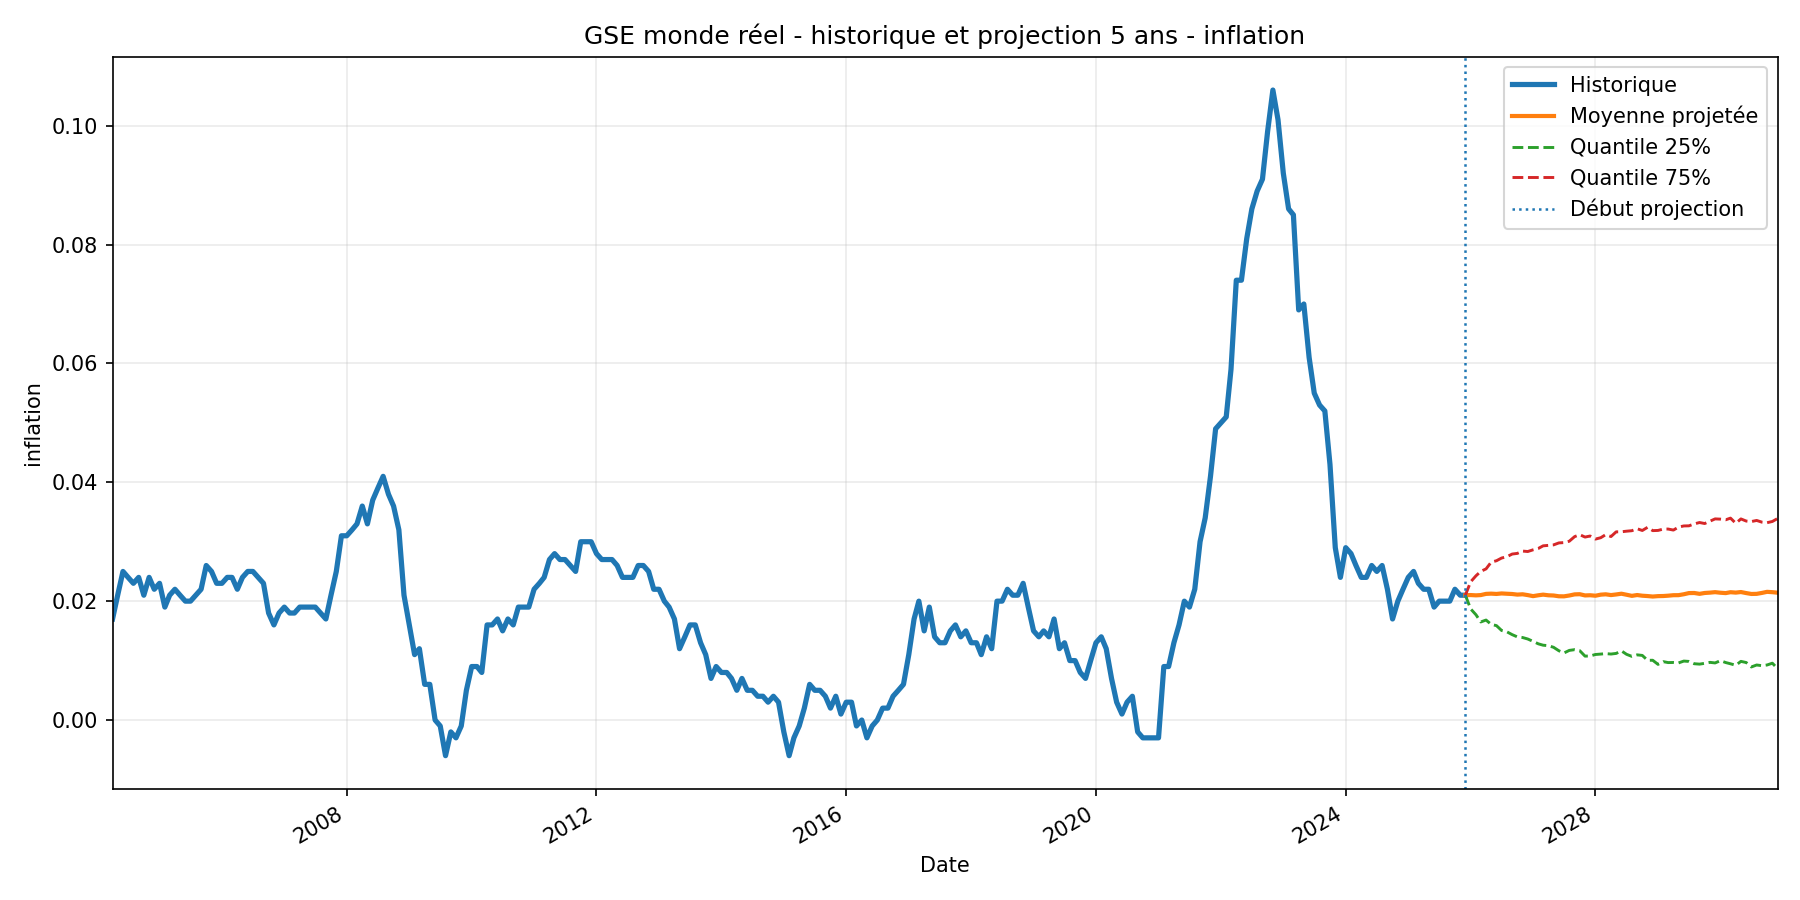
\includegraphics[width=\textwidth]{images/inflation_france_MCO.png}
    \caption{Projection de l'inflation française sur 5 ans (MCO)}
    \label{fig:inflation_france_MCO}
\end{figure}

Cette figure illustre avec la moyenne projetée (en orange), la politique monétaire de la BCE visant un ancrage de l'inflation autour de 2\,\% à long terme. On remarque cependant que cette moyenne reste supérieur au seuil de 2\,\% sur l'horizon de projection. Cela est surement dû à la période de forte inflation post-Covid (2022-2023) qui a influencé le calibrage par MCO. Les quantiles 25\,\% et 75\,\% montrent la dispersion des scénarios simulés, qui s'élargit avec l'horizon de projection, traduisant l'incertitude croissante sur l'évolution future de l'inflation.

\begin{figure}[H]
    \centering
    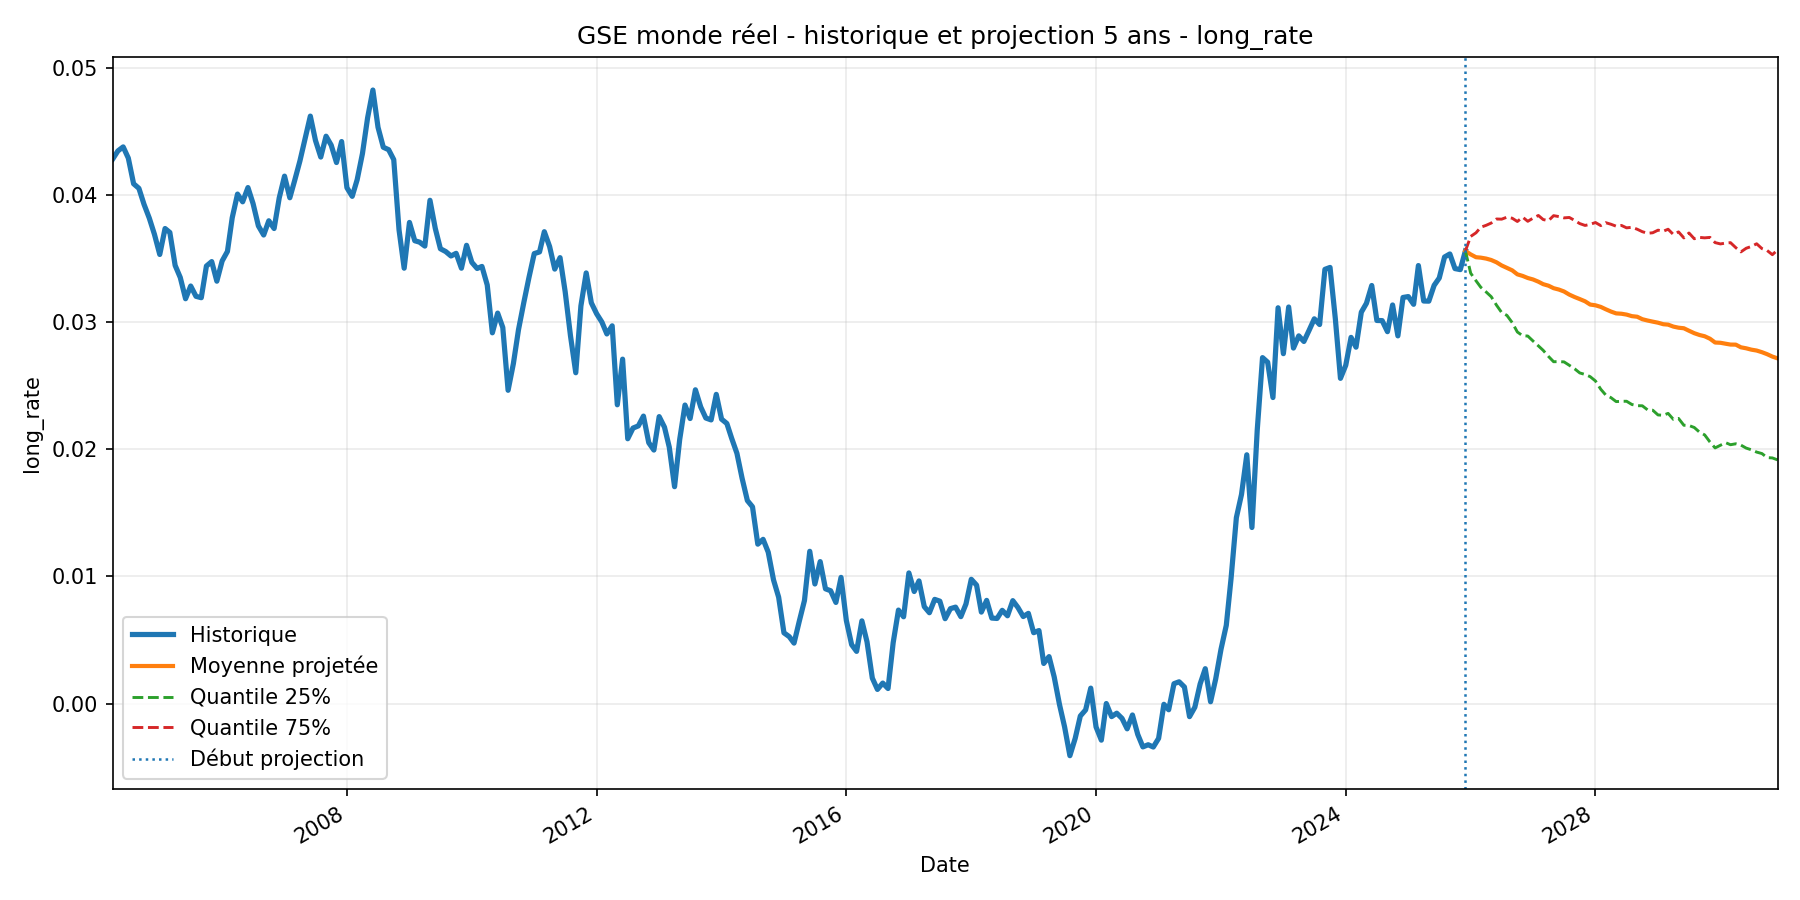
\includegraphics[width=\textwidth]{images/long_rate_MCO.png}
    \caption{Projection du taux long sur 5 ans (MCO)}
    \label{fig:long_rate_MCO}
\end{figure}

Le graphique (figure \ref{fig:long_rate_MCO}) montre la projection du taux long (10 ans) sur 5 ans, avec la moyenne projetée (en orange). On observe que la moyenne projetée diminue rapidemment. Cela est cohérent avec le calibrage par MCO, qui a été influencé par la période de taux bas. Cependant, cela crée aussi une forte rupture avec la tendance actuelle. On se demandera par la suite si ce calibrage est pertinent pour être utilisé comme témoin, ou si un calibrage par expert serait plus approprié pour refléter les objectifs de politique monétaire de la BCE.

\begin{figure}[H]
    \centering
    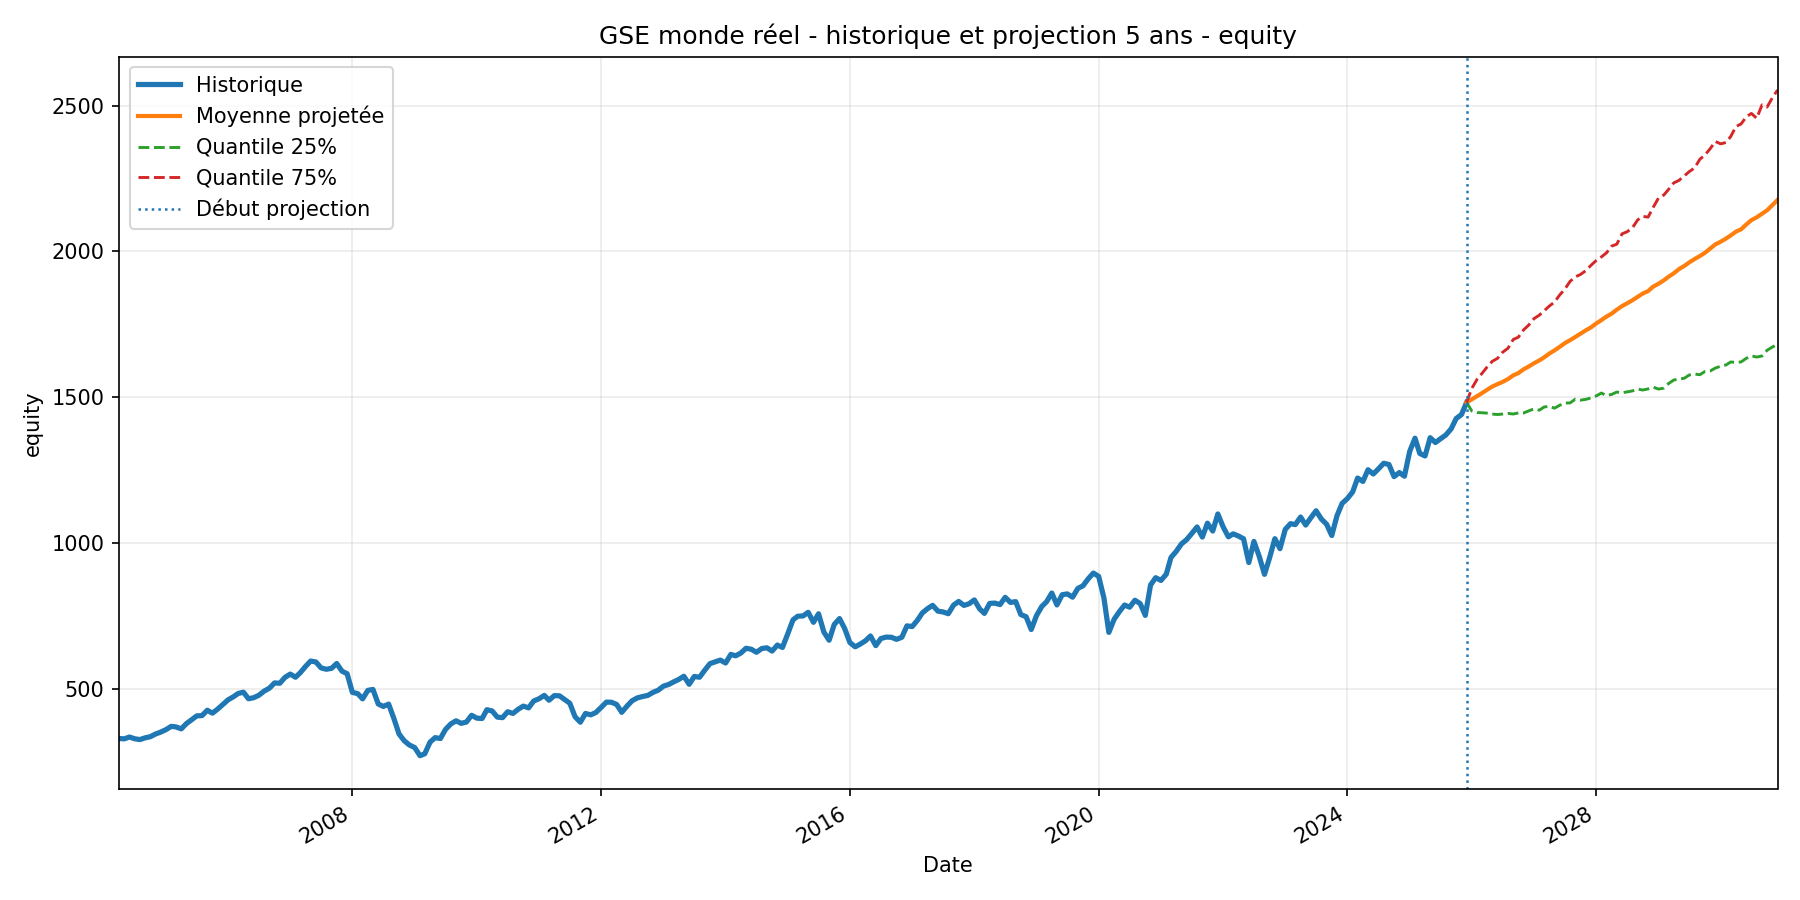
\includegraphics[width=\textwidth]{images/actions_stoxx600NR_MCO.png}
    \caption{Projection du prix du STOXX 600 NR sur 5 ans (MCO)}
    \label{fig:actions_stoxx600NR_MCO}
\end{figure}

Ici, on voit que la moyenne projetée du prix du STOXX 600 NR (en orange) suit une tendance fortement haussière, reflétant la dérive positive estimée à partir des données historiques. On observe que la tendance haussière est très marquée, avec une dispersion des scénarios qui s'élargit plus que pour l'inflation, ce qui est cohérent avec les paramètres estimés : les actions présentent une volatilité 10 fois plus élevée que l'inflation.

\subsection{Résultats du modèle ALM par scénario de calibrage MCO}

Cette sous-section présente les résultats du premier run ALM, alimenté par les 1\,000 trajectoires issues du GSE calibré par MCO sur la période 2004-2025. Les indicateurs analysés successivement sont le taux de rendement des actifs (TRA), le taux servi et le mécanisme de participation aux bénéfices, les rachats, ainsi que les marges financière et d'acquisition.

\subsubsection{Présentation du portefeuille initial}

Le portefeuille servant de base au run ALM est un fonds en euros stylisé dont les conditions initiales sont présentées dans cette section. L'actif total s'élève à 73,5 M€ en valeur nette comptable (VNC), équilibré au passif par une provision mathématique (PM) de 70 M€, une provision pour participation aux excédents (PPE) de 2,8 M€ (soit 4\,\% de la PM) et une réserve de capitalisation (RC) de 0,7 M€ (soit 1\,\% de la PM).

Au bilan d'un fonds en euros, les actifs coexistent sous deux valeurs. La valeur nette comptable (VNC) est la valeur d'entrée inscrite au bilan comptable, nette des amortissements et des provisions pour dépréciation ; elle détermine notamment les revenus obligataires courus et les dotations à la réserve de capitalisation lors des cessions. La valeur de marché (VM) reflète quant à elle la valeur de liquidation courante aux prix de marché ; c'est elle qui conditionne l'allocation réelle du portefeuille au regard des cibles d'investissement. L'écart entre ces deux valeurs, rapporté à la VNC, constitue le taux de plus ou moins-values latentes (PMVL), notion centrale dans la gestion ALM.

La poche obligataire domine largement le bilan, représentant 72\,\% de l'actif en VNC et 66\,\% en valeur de marché (VM). Elle est répartie à parts presque égales entre obligations souveraines françaises (Govies, 26,46 M€ VNC) et obligations corporate (26,46 M€ VNC), avec un spread de 200 points de base appliqué aux secondes. Les actifs risqués représentent 25\,\% de l'actif en VNC, répartis entre deux poches actions (type 1 : 8,27 M€, représentant 75\,\% de la poche actions, et type 2 : 2,76 M€, soit les 25\,\% restants) et une poche immobilier (7,35 M€, soit 10\,\% de l'actif). Le solde, 2,21 M€ (3\,\%), est investi en cash.

L'allocation cible, exprimée en valeur de marché, est la suivante : obligations 66,1\,\% (dont 48,5\,\% de souverains et 51,5\,\% de corporate au sein de la poche), actions 18,8\,\% (type 1 : 14,1\,\%, type 2 : 4,7\,\%), immobilier 12,1\,\% et cash 3,0\,\%. Le portefeuille initial est très proche de cette cible en VM ; le léger écart entre VNC et VM sur les différentes poches s'explique par la situation des plus ou moins-values latentes.


La situation des PMVL au démarrage de la projection est contrastée. Les obligations sont en moins-values latentes significatives : $-$11,5\,\% pour les souverains et $-$5,9\,\% pour le corporate, traduisant le fait que les obligations acquises à des taux bas sont désormais dépréciées par la remontée des taux directeurs de la BCE amorcée en 2022. À l'inverse, les actifs risqués présentent des plus-values latentes notables : 25\,\% sur les actions et 20\,\% sur l'immobilier. Le taux global de PMVL s'établit à $-$0,5\,\%, traduisant une quasi-neutralité de la position latente d'ensemble, les moins-values obligataires étant largement compensées par les plus-values sur actifs risqués. Cette configuration n'est pas sans conséquence pour la gestion ALM : toute cession obligataire en cours de projection réalisera une moins-value absorbée par la réserve de capitalisation, tandis que les cessions d'actifs risqués alimenteront le mécanisme de \textit{turnover} décrit en section~\ref{sec:structure_alm}.

La PPE de 2,8 M€ place le fonds dans une position intermédiaire : elle est loin de la limite réglementaire de 10\,\% des PM comme de l'épuisement total, ce qui lui confère une capacité de dotation et de reprise significative au cours de la projection. La RC de 0,7 M€ reste relativement mince et pourrait constituer une contrainte en cas de cessions obligataires importantes en début de projection. Le taux servi en N$-$1 est de 2,64\,\%, légèrement supérieur au taux cible de 2,50\,\% constaté la même année ; ce point de départ conditionne le mécanisme de PB dès la première année de projection via la composante 80\,\% du taux servi précédent dans la formule du taux cible.

\subsubsection{Taux de rendement des actifs (TRA)}

Le taux de rendement des actifs (TRA) agrège l'ensemble des revenus financiers du portefeuille que sont les coupons obligataires, les dividendes et les revenus locatifs capitalisés ainsi que les plus-values réalisées. Cet ensemble est rapporté à la valeur nette comptable de l'actif. C'est le TRA qui alimente le mécanisme de participation aux bénéfices décrit en section~\ref{sec:structure_alm} : il constitue donc la variable de transmission centrale entre la performance du portefeuille et le taux servi aux assurés. La figure~\ref{fig:TRA_MCO} représente la distribution du TRA sur les 40 années de projection sous le calibrage MCO, à travers les quantiles P5, P25, P75 et P95 ainsi que la moyenne.

\begin{figure}[H]
    \centering
    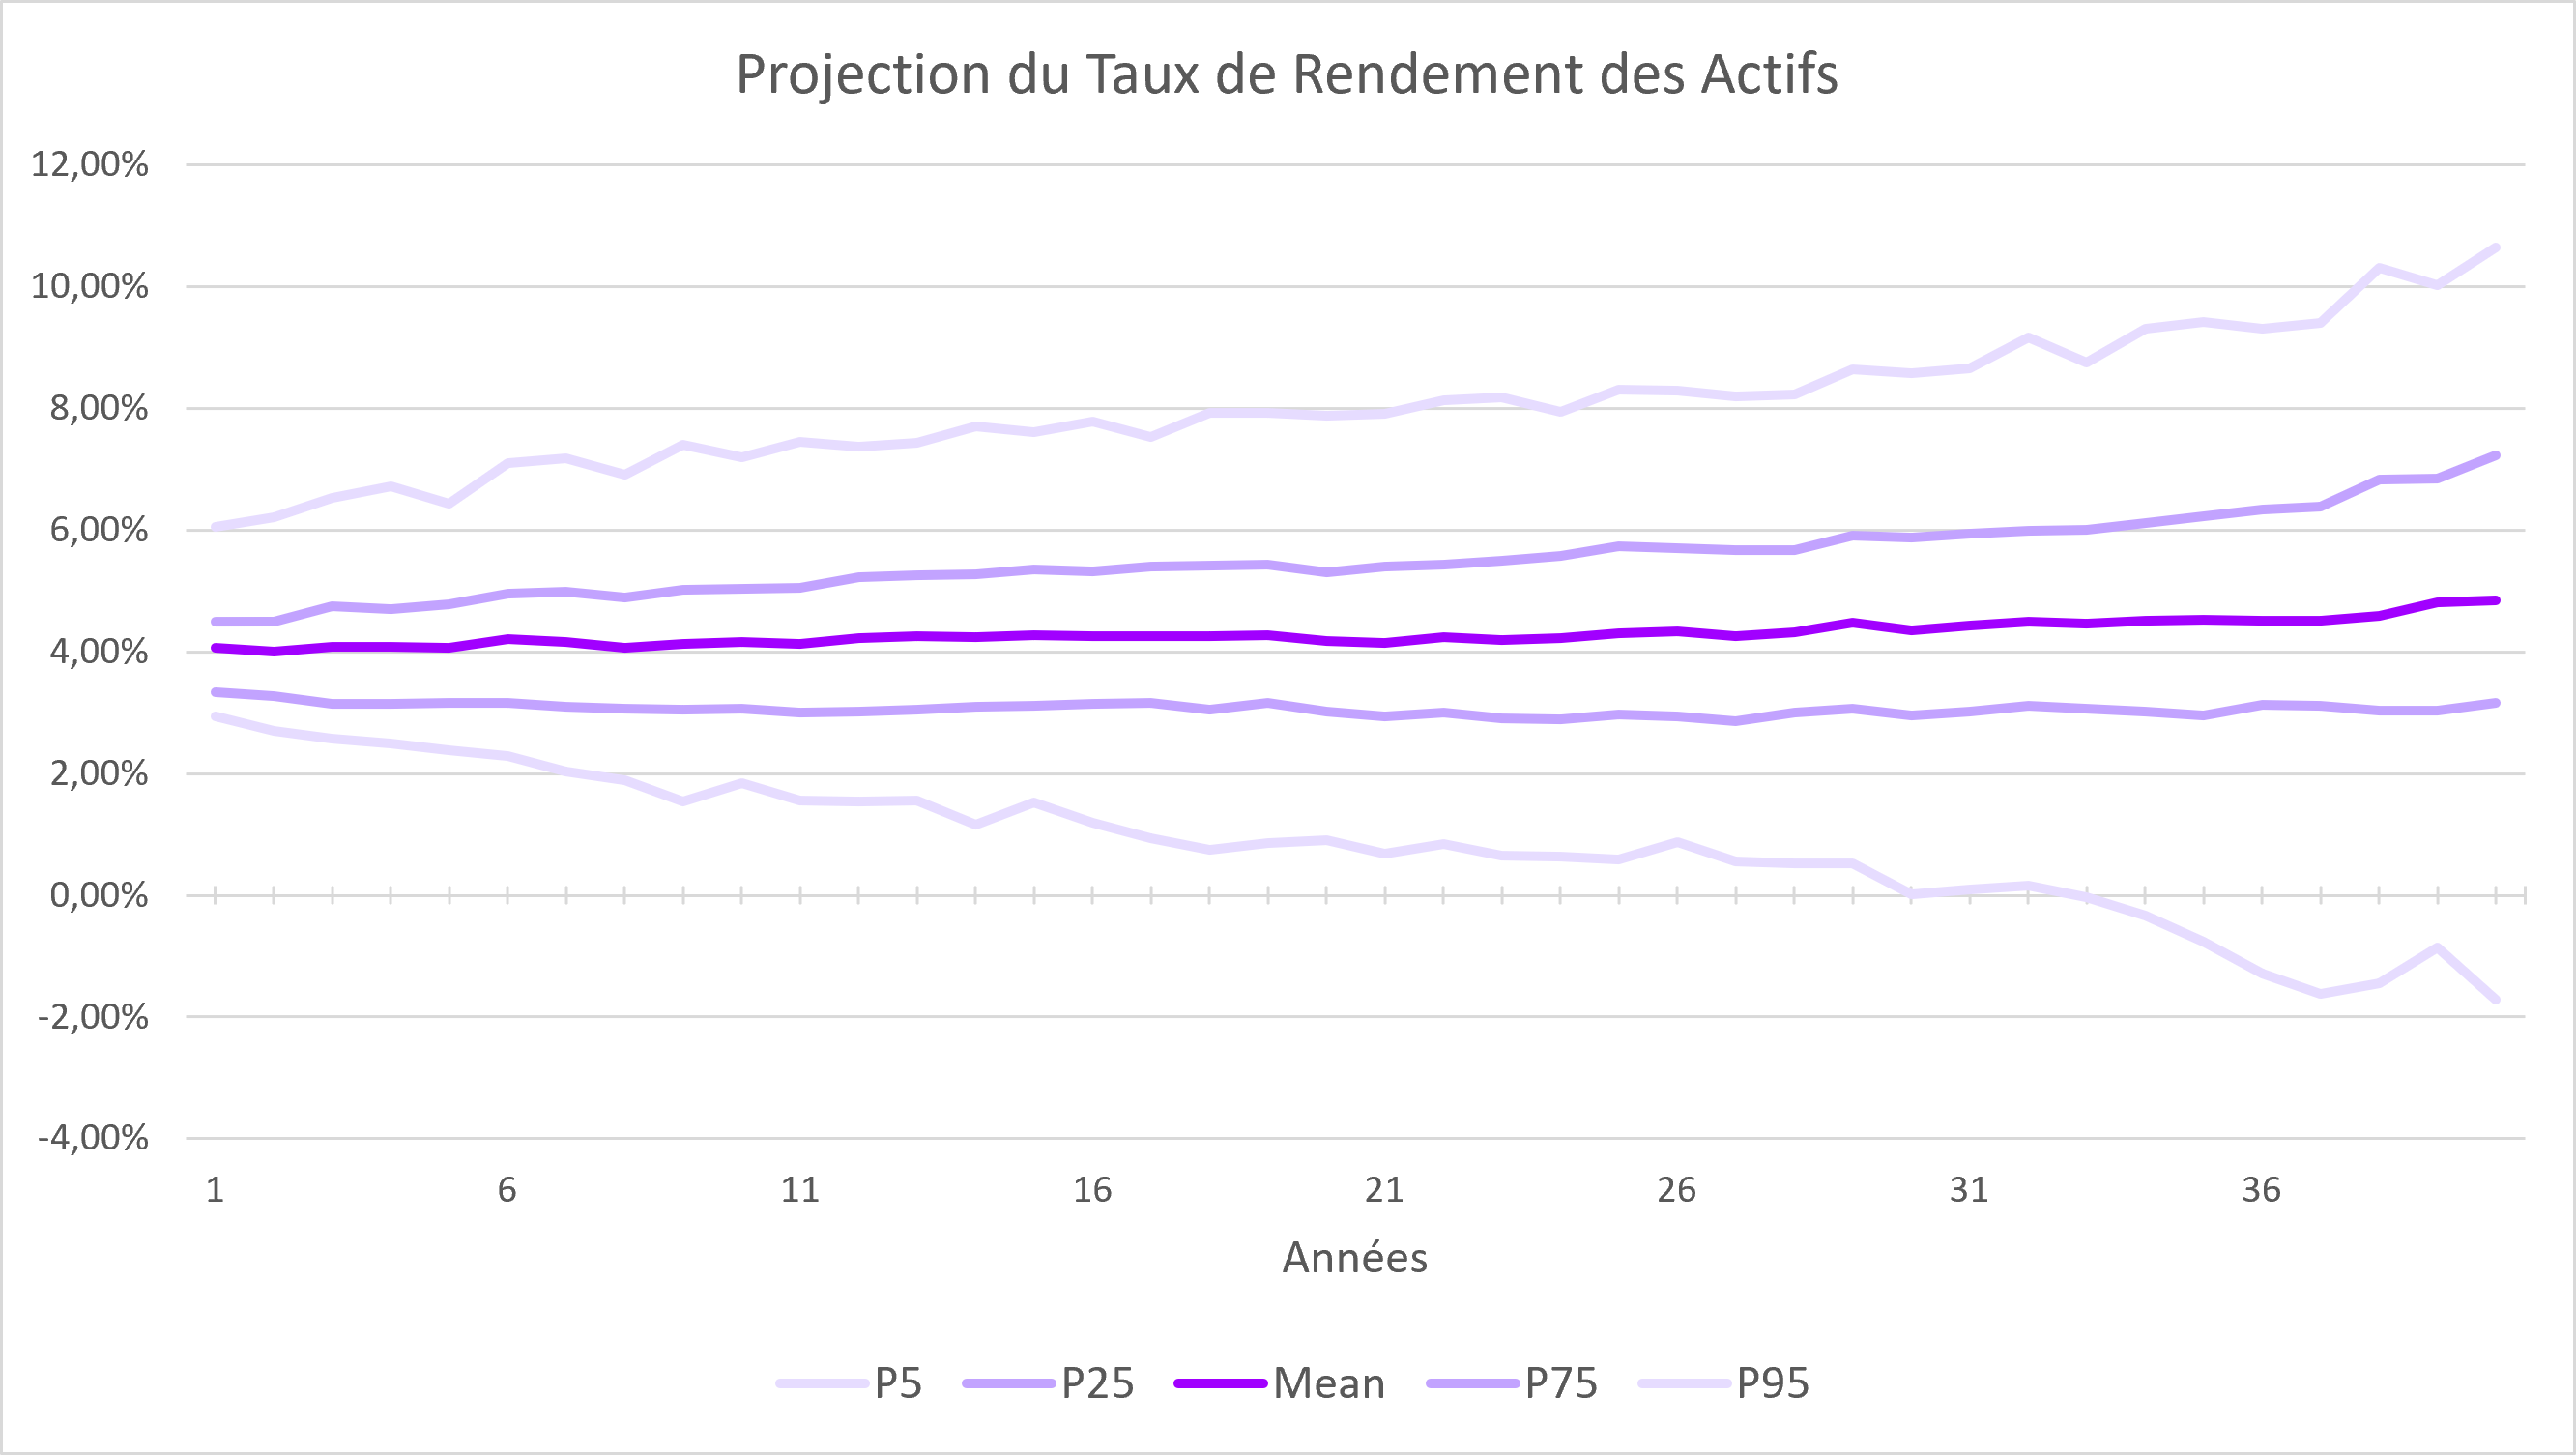
\includegraphics[width=\textwidth]{images/TRA_MCO.png}
    \caption{Distribution du TRA sur 40 ans}
    \label{fig:TRA_MCO}
\end{figure}


Le TRA moyen reste remarquablement stable sur l'ensemble de l'horizon, oscillant entre 4,0\,\% et 4,9\,\% selon les années de projection. La légère hausse de la moyenne en fin d'horizon (4,85\,\% en an 40) traduit le renouvellement progressif du portefeuille obligataire vers les niveaux de long terme estimés par le GSE ($\hat{\theta}_{10y} = 2{,}02\,\%$ contre des taux initiaux inférieurs), ainsi que la capitalisation des plus-values sur actifs risqués dans les scénarios médians.

L'intervalle interquartile P25--P75 s'élargit progressivement, passant de 1,2 point de pourcentage en an~1 à 4,1 points en an~40. La fourchette totale P5--P95 suit la même tendance, de 3,1 points en an~1 à 12,4 points en an~40. Cet élargissement reflète l'accumulation de l'incertitude sur les trajectoires de taux d'intérêt et la volatilité des actifs risqués : plus l'horizon s'éloigne, plus les écarts entre scénarios favorables et défavorables se creusent.

Le percentile 5 (P5), initialement à 2,94\,\%, se dégrade régulièrement pour devenir négatif à partir de l'an~33 et atteindre $-$1,71\,\% en an~40. Ces scénarios défavorables correspondent à une combinaison de taux bas persistants, réduisant le rendement des obligations nouvellement émises lors des renouvellements successifs, et de corrections des actifs risqués, qui compriment le TRA global jusqu'à le rendre négatif. Un TRA négatif signifie que les pertes réalisées sur cessions d'actifs excèdent les revenus courants du portefeuille ; c'est une situation extrême qui met en tension les mécanismes de redistribution du modèle ALM, en particulier la PPE et la réserve de capitalisation.

La distribution présente une asymétrie positive marquée à long terme : le P95 gagne environ 4,6 points de pourcentage entre l'an~1 et l'an~40 (de 6,1\,\% à 10,6\,\%), tandis que le P5 se dégrade d'un montant comparable dans l'autre sens. Cette asymétrie est structurelle et reflète la nature des mouvements browniens géométriques sous-jacents aux actifs risqués : leur dérive positive génère, dans les bons scénarios, une accumulation croissante de plus-values sans borne supérieure, tandis que les pertes en valeur de marché demeurent bornées par la valeur plancher des actifs.

\subsubsection{Comparaison entre le TRA et le taux servi}

On s'attend à avoir un taux servi moyen inférieur au TRA moyen. En effet, le TRA mesure ce que l'actif rapporte et le taux servi mesure ce qui en est effectivement restitué à l'assuré après marge de l'assureur, frais et politique de lissage. La figure \ref{fig:tra_vs_tx_servi_mco} compare les distributions du TRA et du taux servi sur l'horizon de projection.

\begin{figure}[H]
    \centering
    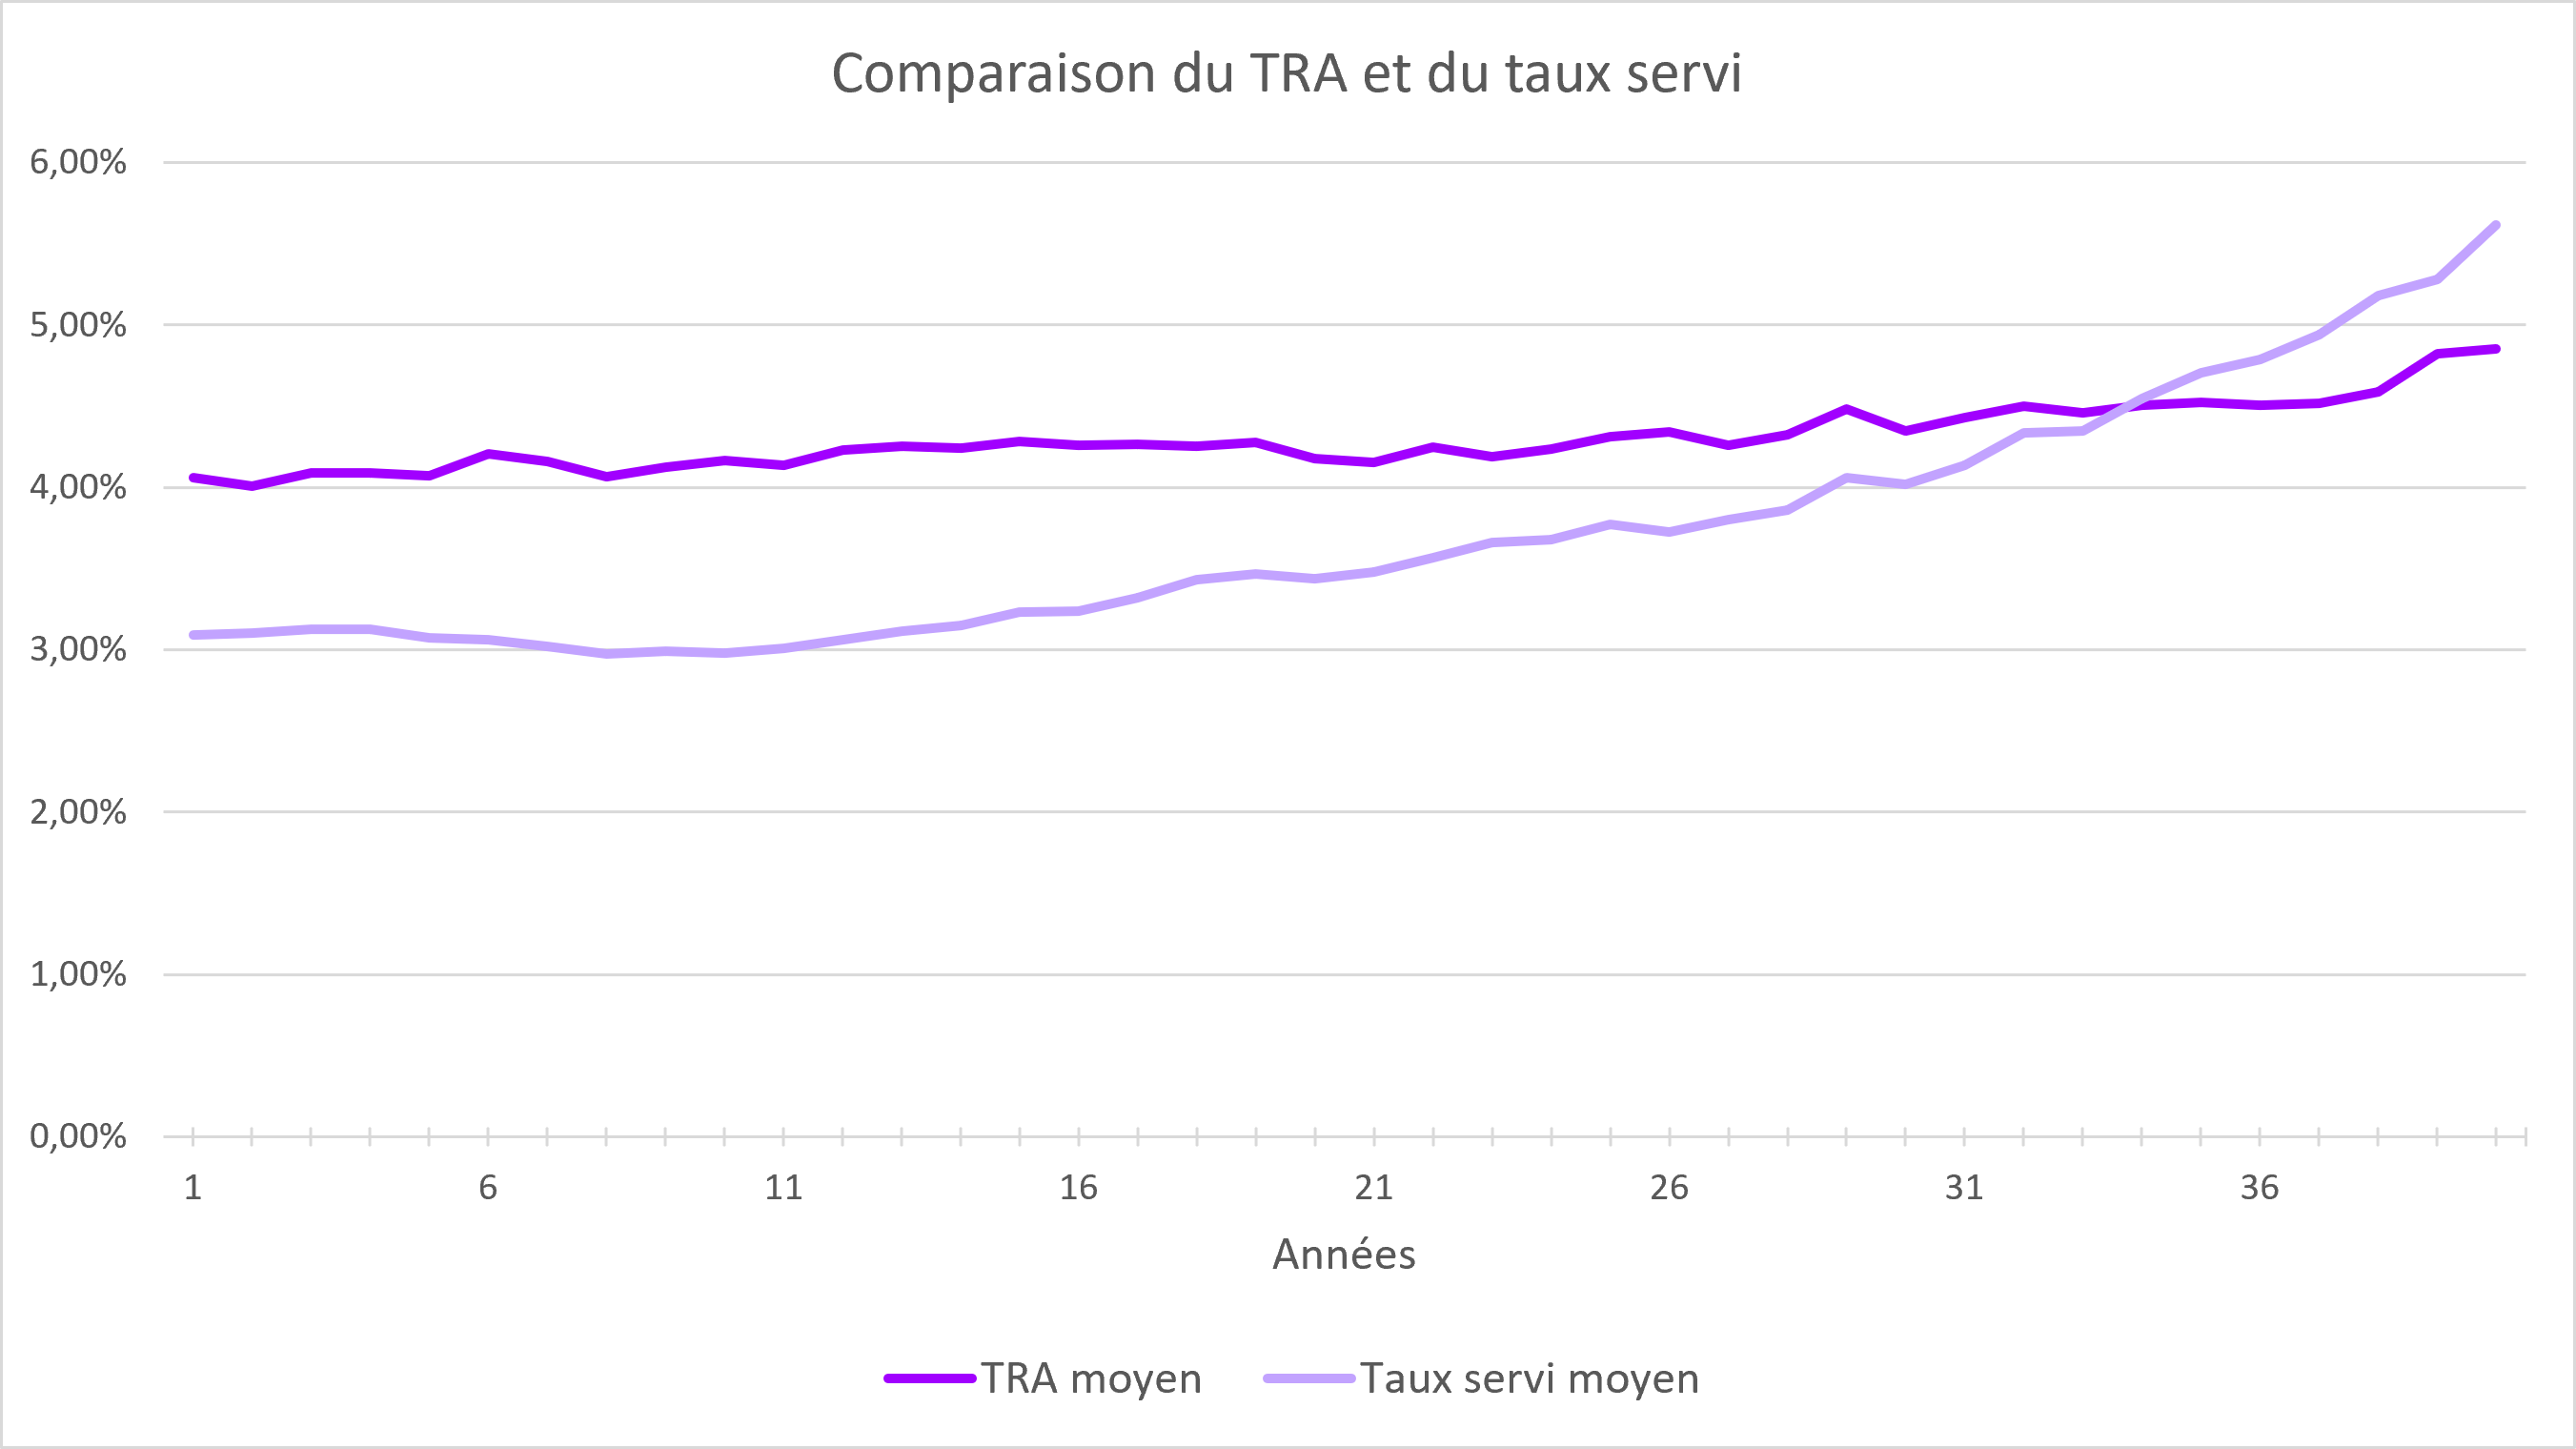
\includegraphics[width=\textwidth]{images/tra_vs_tx_servi_mco.png}
    \caption{Comparaison entre le TRA et le taux servi sur 40 ans}
    \label{fig:tra_vs_tx_servi_mco}
\end{figure}

On remarque que notre attente est vérifiée sur les 15 / 20 premières années, avec un taux servi moyen inférieur au TRA moyen. Les deux courbes suivent globalement une trajectoire similaire. Cependant, à partir de l'an 20, le taux servi moyen ammorce une hausse plus rapide que le TRA moyen, jusqu'à dépasser ce dernier vers 33 ans. On peut expliquer cette hausse progressive du taux servi par l'effet de la PPE, qui doit être reprise des millésimes anciens. On a aussi le phénomène de plafond de la PPE, qui ne peut pas dépasser 10\% de la PM. La PM diminue chaque année car les sorties dépassent les entrées. En effet, on ne considère pas de flux entrant dans le portefeuille (pas de New Business ni de cotisation) et les flux sortants sont les prestations de rachats et de décès. Ainsi, comme le montre la figure \ref{fig:PPE_MCO}, la PPE est reprise progressivement et massivement à partir de l'an 20, ce qui permet d'augmenter le taux servi.

\begin{figure}[H]
    \centering
    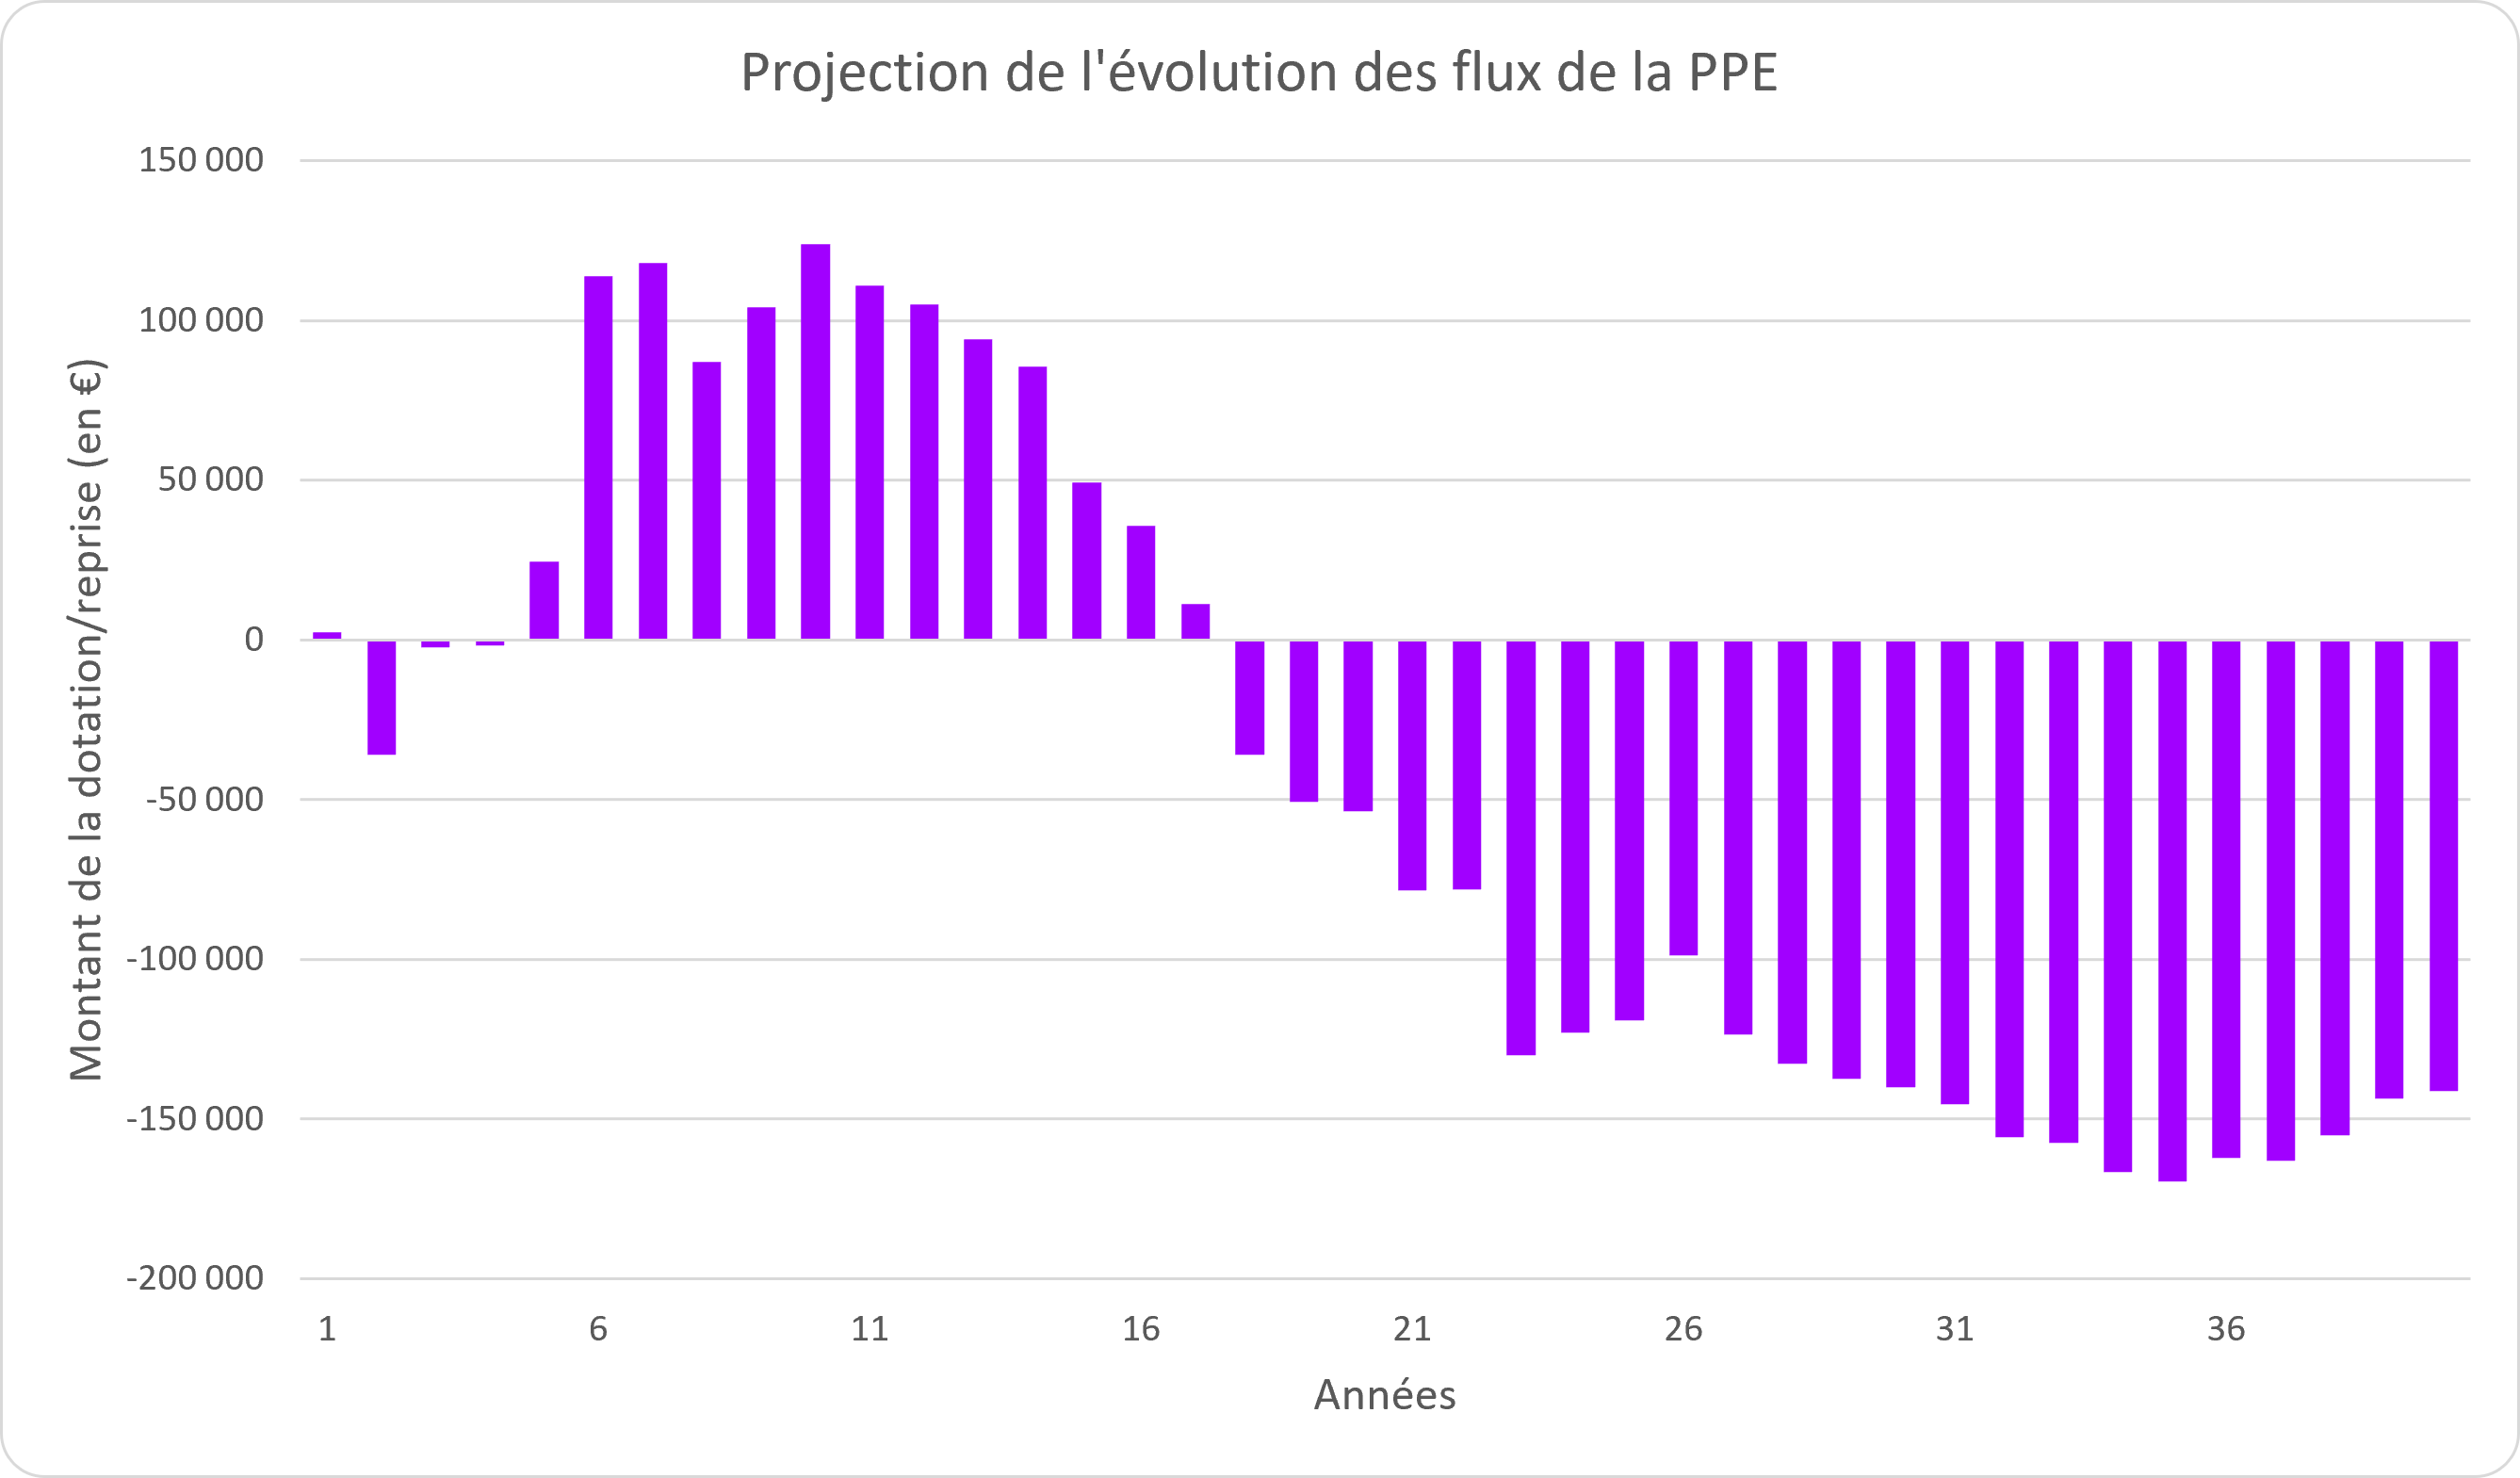
\includegraphics[width=\textwidth]{images/variations_PPE_MCO.png}
    \caption{Flux moyens de dotation et reprise de PPE}
    \label{fig:PPE_MCO}
\end{figure}

En définitive, la comparaison confirme l'intuition initiale sur l'essentiel de l'horizon de projection : le taux servi reste inférieur au TRA tant que la PPE se constitue, matérialisant la part du rendement financier volontairement mise en réserve plutôt que distribuée aux assurés. Le croisement observé à partir de l'an 33 ne contredit pas ce résultat, il en révèle la limite : l'écart entre le TRA et le taux servi n'est pas stable dans le temps, il dépend de la phase du cycle de la PPE. Ce cycle est provoqué par un mécanisme qui absorbe l'écart pendant la phase de constitution, puis le restitue avec retard lors de sa reprise (règle des 8 ans, plafond des 10\% de la PM). Le taux servi observé sur un exercice donné ne peut donc pas s'interpréter isolément comme le reflet du rendement de l'actif de cette même année : il porte, via la PPE, la mémoire des écarts cumulés des exercices précédents. Cela explique que la hiérarchie attendue entre TRA et taux servi finisse par s'inverser sur le long terme. 
Une autre conséquence de la hausse progressive du taux servi est la création d'un décalage inter-générationnel entre assurés. La PPE constituée au profit d'une cohorte de contrats peut n'être reversée que des années plus tard, au bénéfice des seuls assurés encore présents à cette date donc ceux qui rachètent ou décèdent entre-temps ne perçoivent jamais leur part de la richesse qu'ils ont pourtant contribué à générer.

\subsubsection{Rachats}

Le montant des rachats reste élevé sur les 5-6 premières années avant de diminuer progressivement jusqu'à devenir quasi nul en fin de projection. Cette baisse de long terme s'explique par la fonte de la PM : le portefeuille est fermé, sans new business ni cotisation, donc l'assiette sur laquelle s'applique le taux de rachat se réduit chaque année, entraînant mécaniquement celle des montants rachetés.

Le plateau initial (figure \ref{fig:prestations_rachat_euro_mco}), lui, s'explique par la composante conjoncturelle du rachat : au taux de rachat structurel s'ajoute un ajustement dynamique fonction de l'écart entre le taux servi de l'année précédente et le TME, qui joue le rôle de taux concurrent. Quand l'assureur sert moins que le marché, les assurés rachètent davantage ; quand il sert plus, les rachats diminuent. Or on a montré que le taux servi reste en retrait du TRA (et donc du TME) sur les premières années, le temps que le mécanisme de lissage rattrape son retard : cet écart défavorable alimente des rachats conjoncturels supplémentaires, ce qui maintient les montants rachetés à un niveau élevé avant que l'effet de base, la décroissance continue de la PM, ne devienne dominant à partir de l'année 6-7.

\begin{figure}[H]
    \centering
    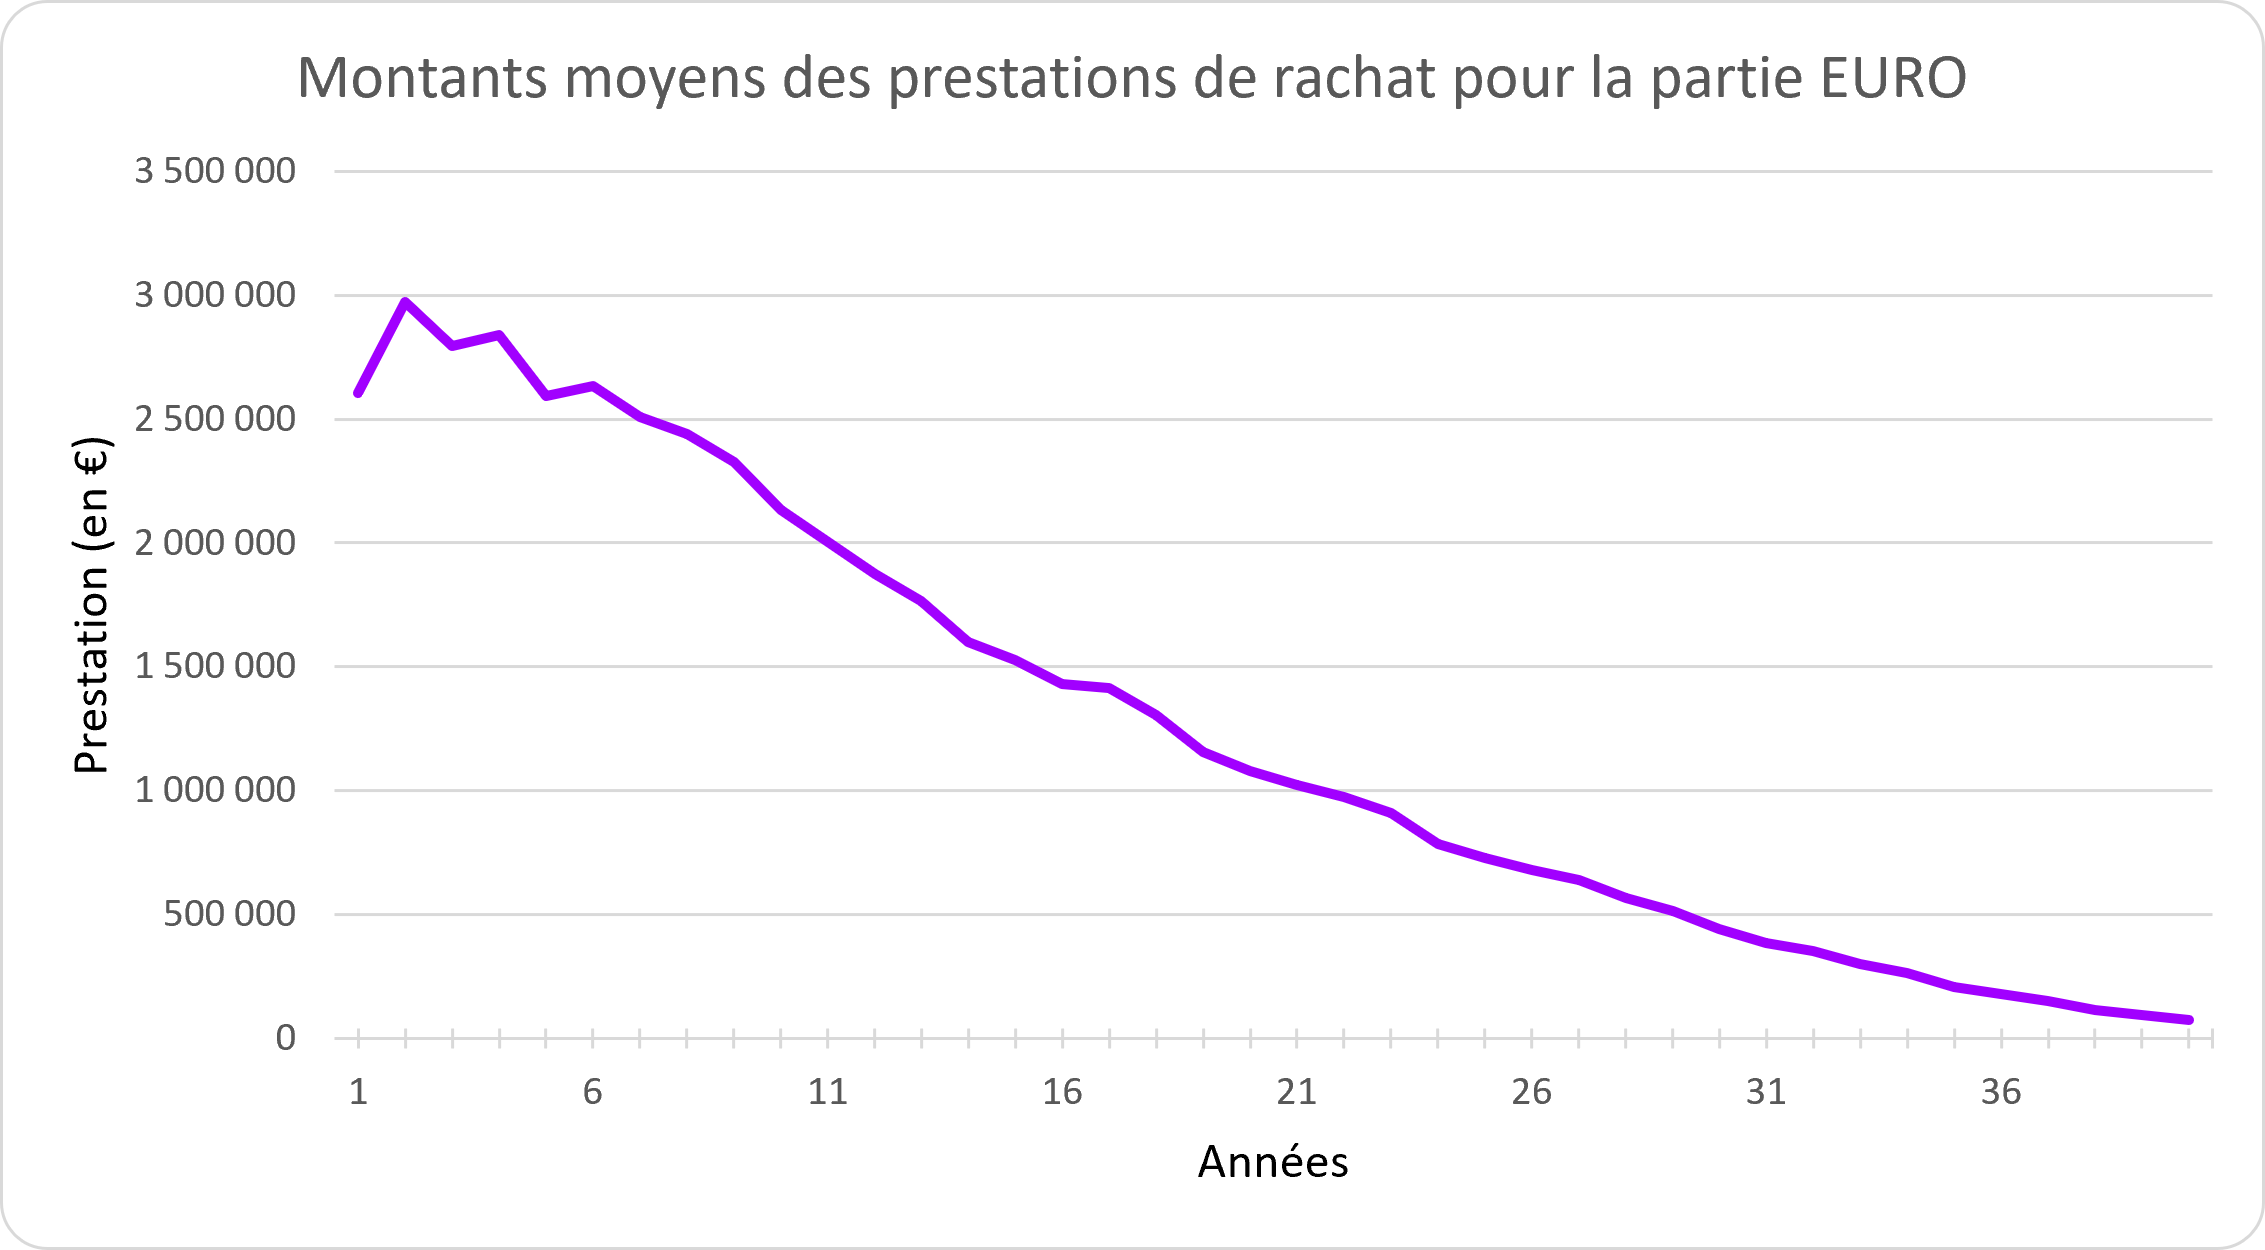
\includegraphics[width=\textwidth]{images/prestations_rachat_euro_mco.png}
    \caption{Projection des prestations de rachats sur 40 ans, partie EURO}
    \label{fig:prestations_rachat_euro_mco}
\end{figure}

\subsubsection{Marges}

Le run étant en run-off, les marges d'acquisition sont nulles sur l'ensemble de l'horizon : aucune cotisation ni aucun new business n'entre dans le portefeuille, il n'y a donc ni chargement sur prime perçu ni frais d'acquisition à financer. Nous concentrons donc l'analyse sur la marge financière, représentée par le solde financier.

On observe sur la figure \ref{fig:solde_financier_mco} une baisse progressive et quasi continue du solde financier sur la quasi-totalité de l'horizon, avant un rebond brutal en toute dernière année. Cette décroissance suit directement celle de la PM : le portefeuille étant fermé, l'actif sous gestion diminue chaque année, ce qui réduit d'autant les produits financiers générés et, par ricochet, le solde financier qui en découle.

\begin{figure}[H]
    \centering
    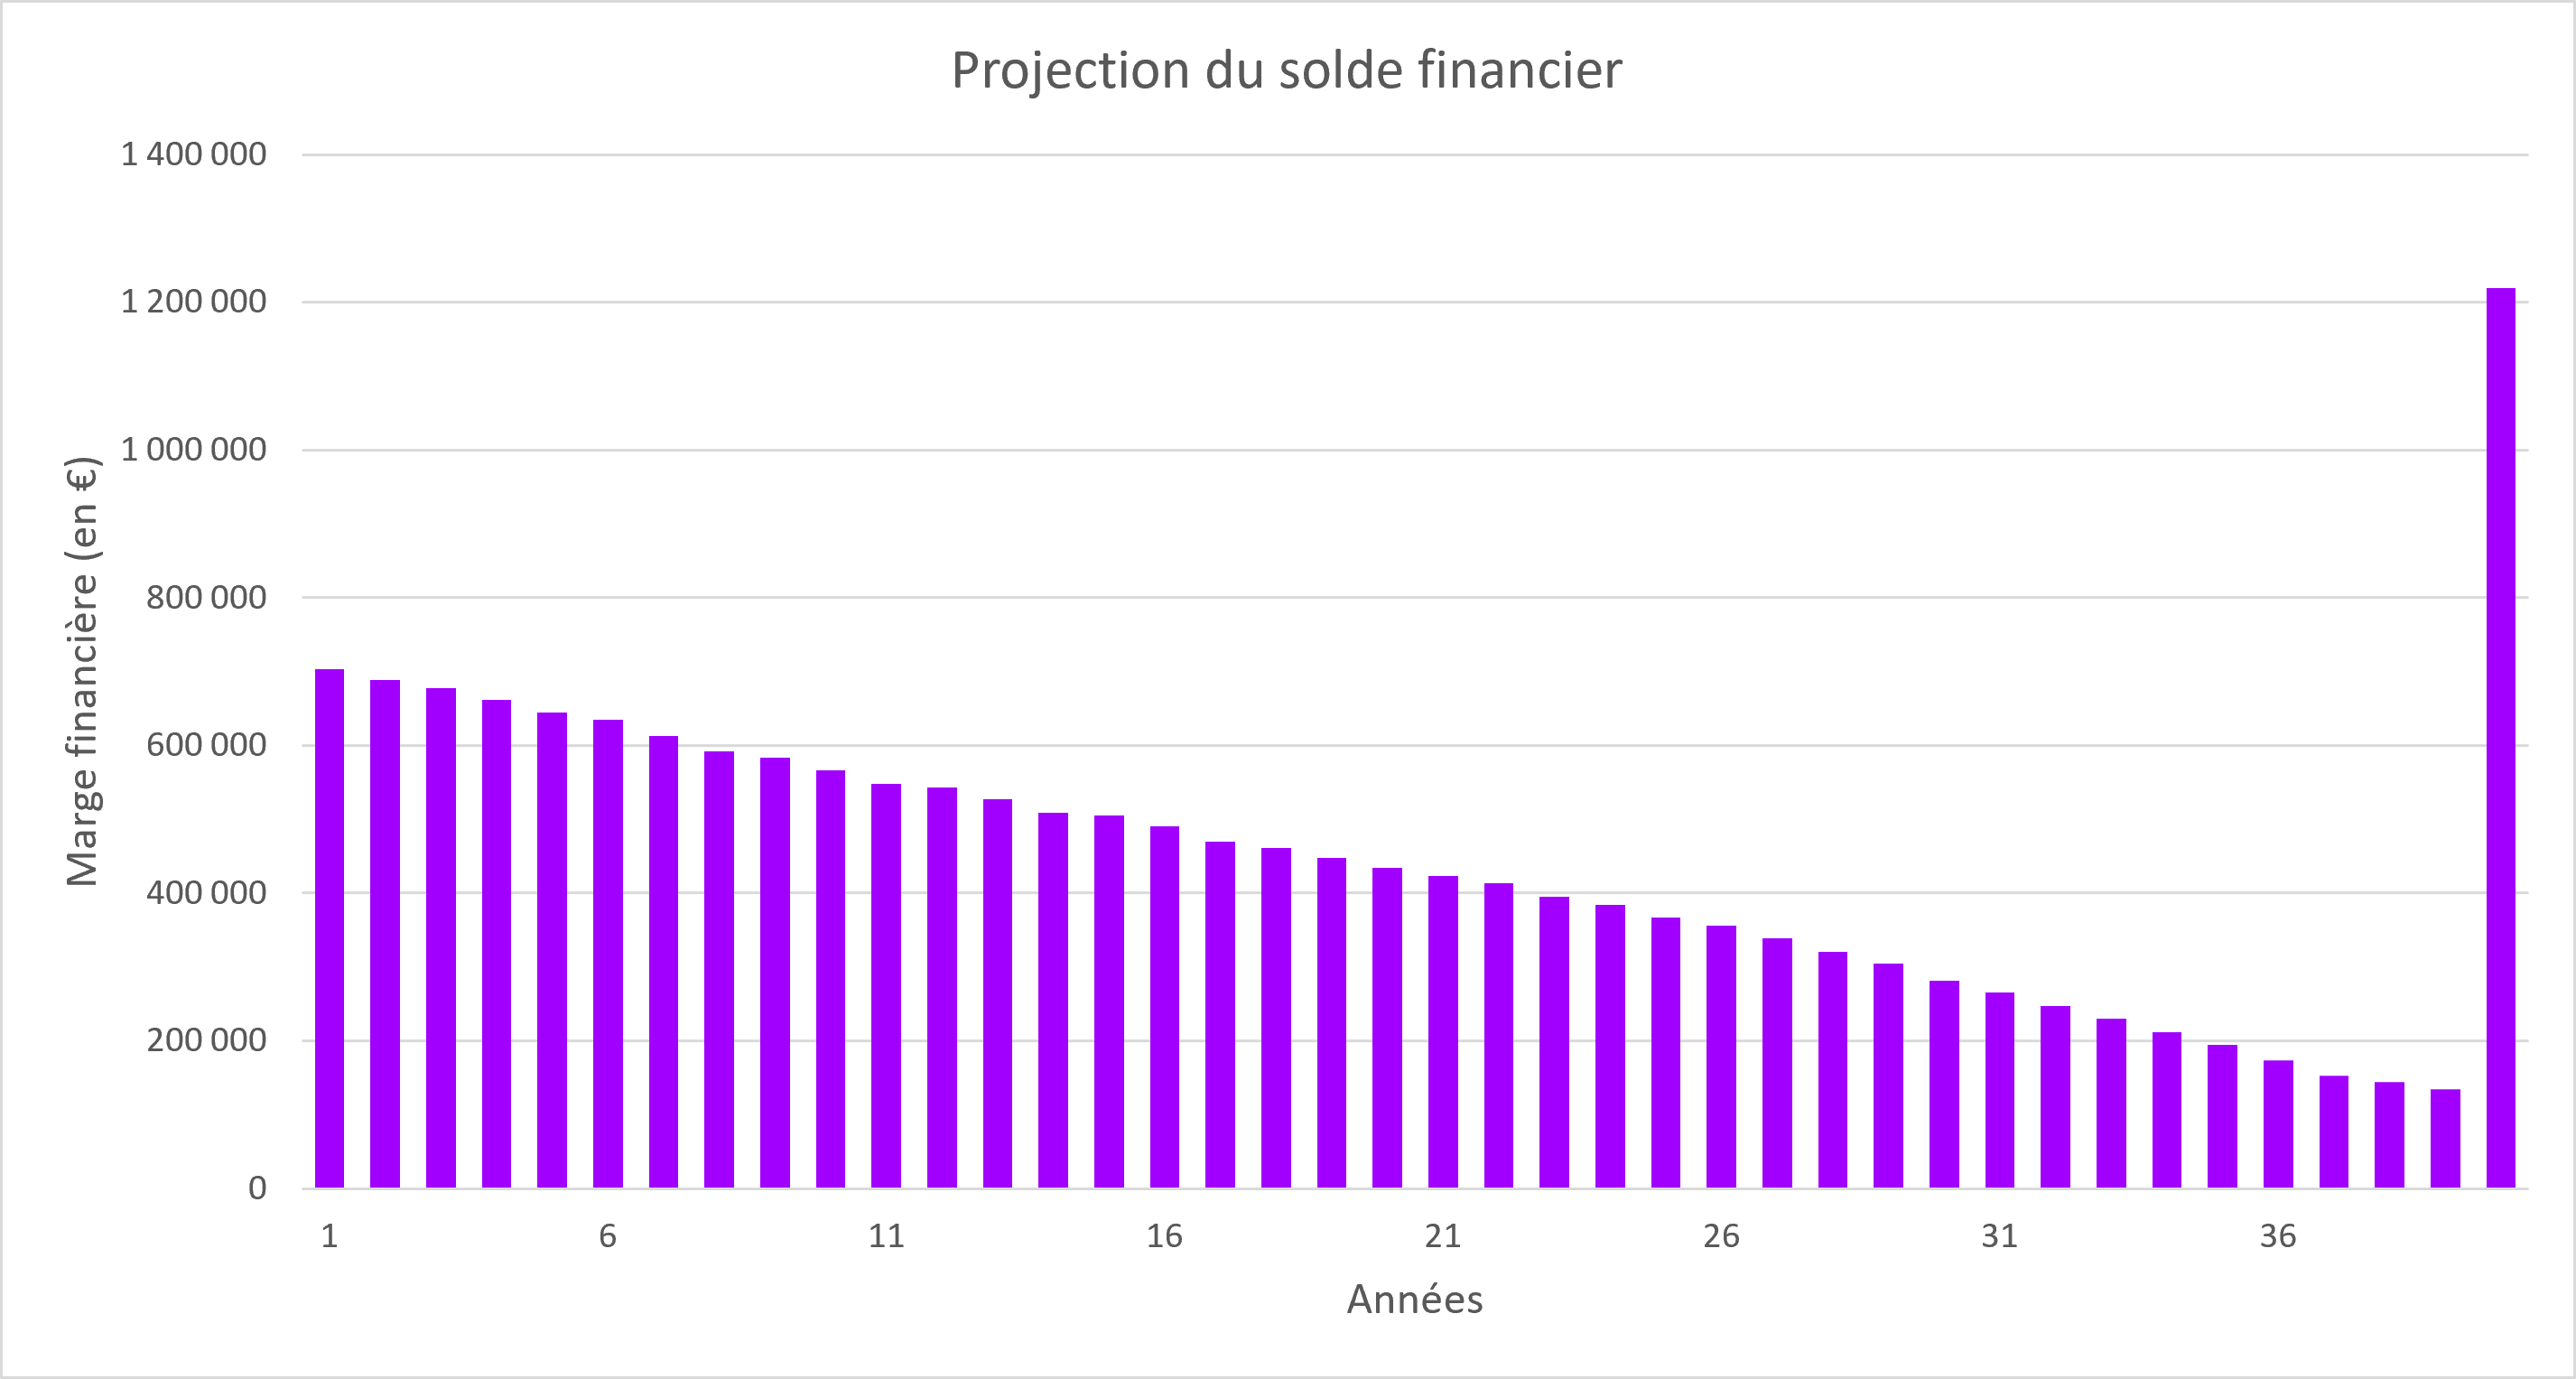
\includegraphics[width=\textwidth]{images/solde_financier_mco.png}
    \caption{Projection du solde financier sur 40 ans}
    \label{fig:solde_financier_mco}
\end{figure}

En année 1 (figure \ref{fig:compo_solde_financier_annee_1_mco}), le solde financier se compose presque exclusivement de deux postes de sens opposé : les produits financiers (2 869 684 €), dont l'essentiel est reversé aux assurés sous forme de PB (-2 154 563 €). Les intérêts techniques (-10 947 €) et les variations de PPE et de RC restent marginaux à ce stade. Le solde financier net qui en résulte (702 886 €) représente ainsi la part des produits financiers conservée par l'assureur après distribution de la participation aux bénéfices, soit environ un quart des produits financiers de l'année.

\begin{figure}[H]
    \centering
    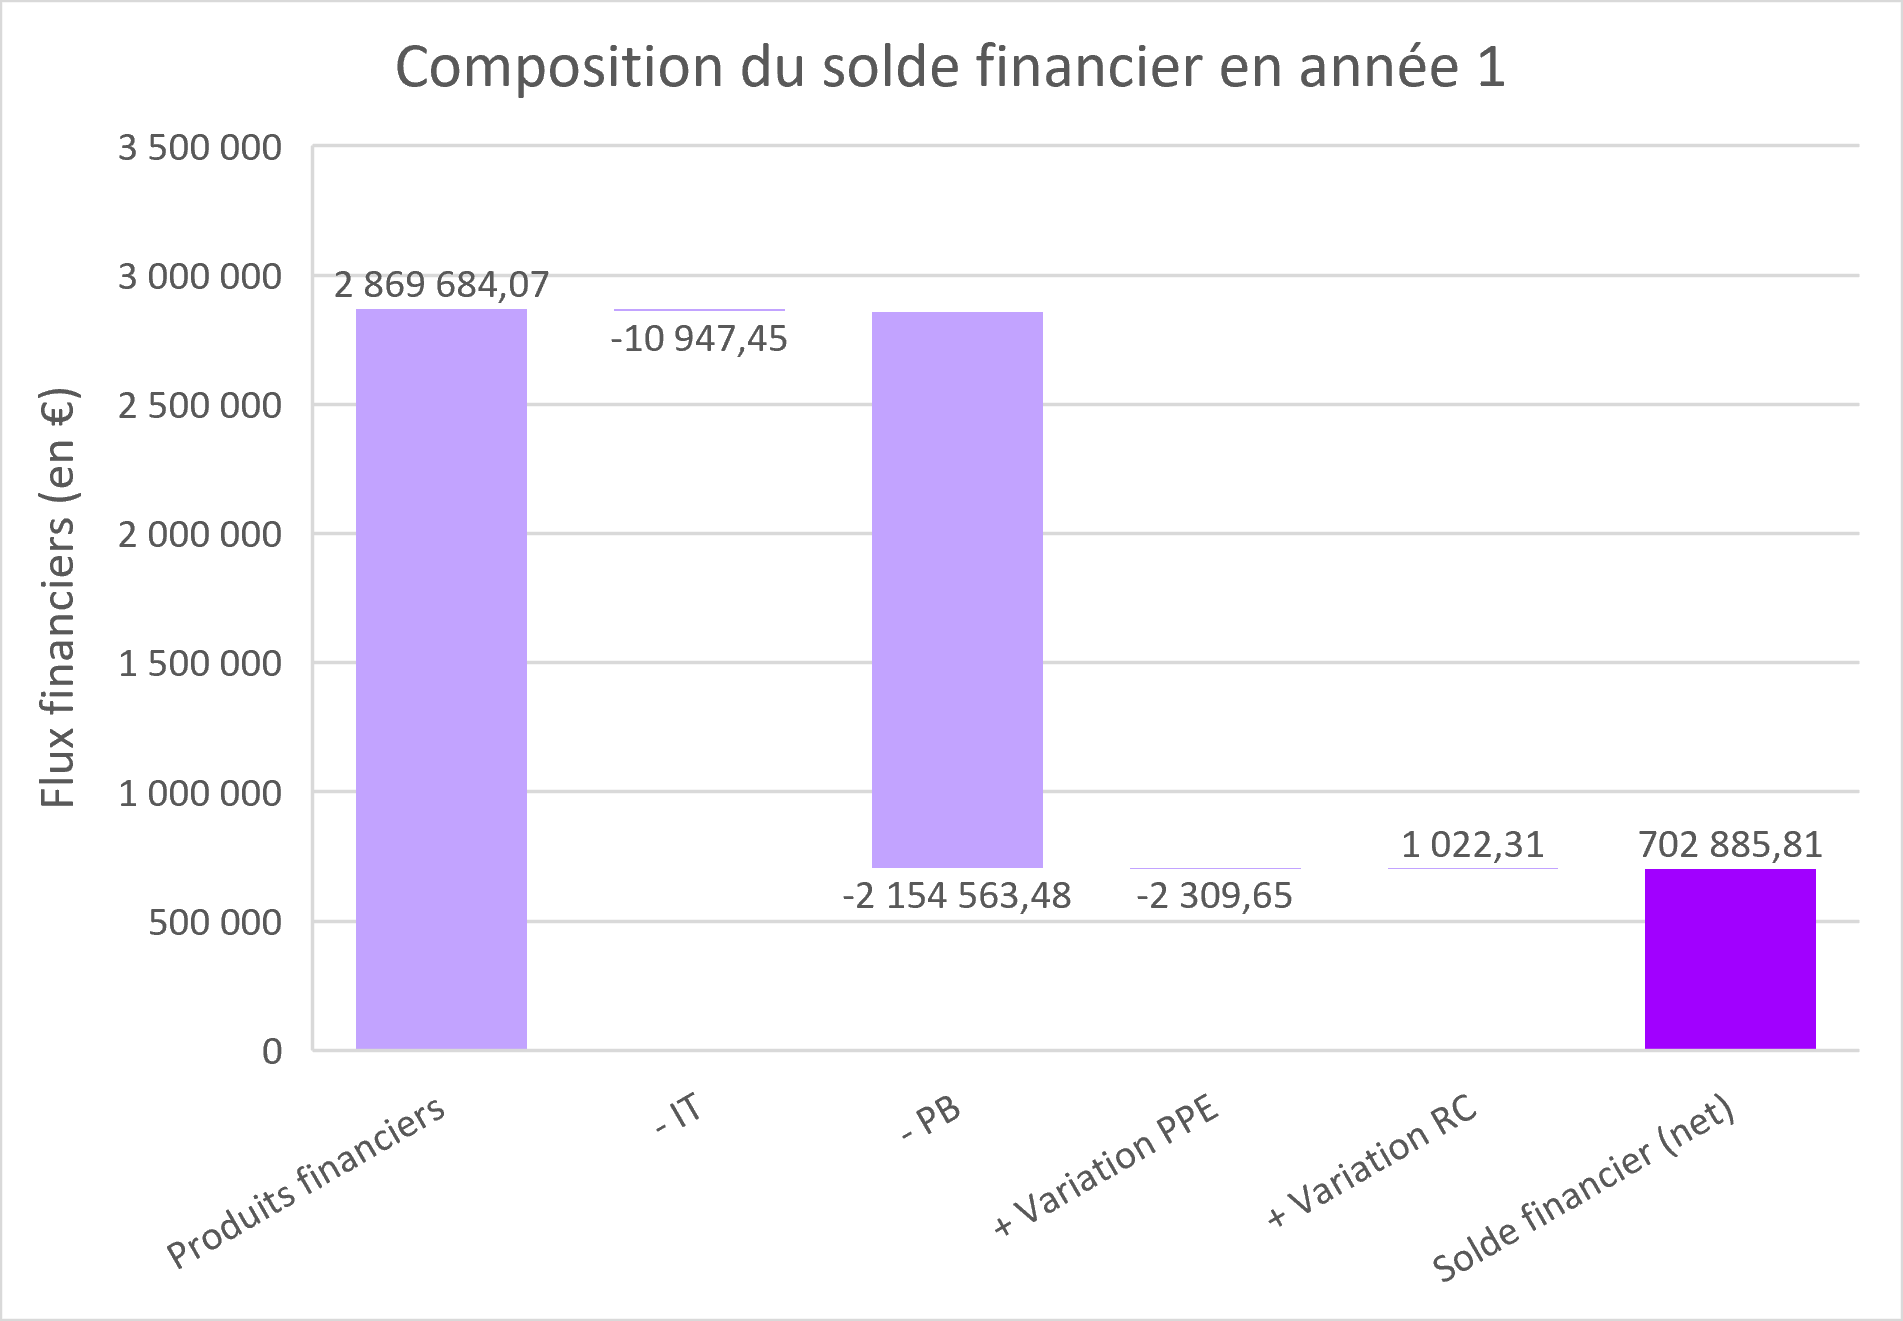
\includegraphics[width=0.65\textwidth]{images/compo_solde_financier_annee_1_mco.png}
    \caption{Composition du solde financier en année 1}
    \label{fig:compo_solde_financier_annee_1_mco}
\end{figure}

En année 40 (figure \ref{fig:compo_solde_financier_annee_40_mco}), la structure est très différente. Les produits financiers récurrents (642 629 €) et la PB qui en découle (-660 379 €) sont mécaniquement plus faibles, à l'image de la PM résiduelle en fin de portefeuille. Mais le solde financier de cette dernière année est en réalité dominé par les ajustements de fin de projection (+1 101 934 €) : la réserve de capitalisation restante, les plus-values latentes sur les obligations, actions et immobilier encore en portefeuille, ainsi qu'une fraction de la PPE non distribuée, sont intégralement reconnues en résultat lors de la liquidation du portefeuille. C'est cet effet ponctuel, sans lien avec la rentabilité récurrente du contrat, qui explique le rebond observé en toute fin de la figure \ref{fig:solde_financier_mco} : il traduit une convention de clôture de la projection, et non une amélioration de la performance financière du portefeuille.

\begin{figure}[H]
    \centering
    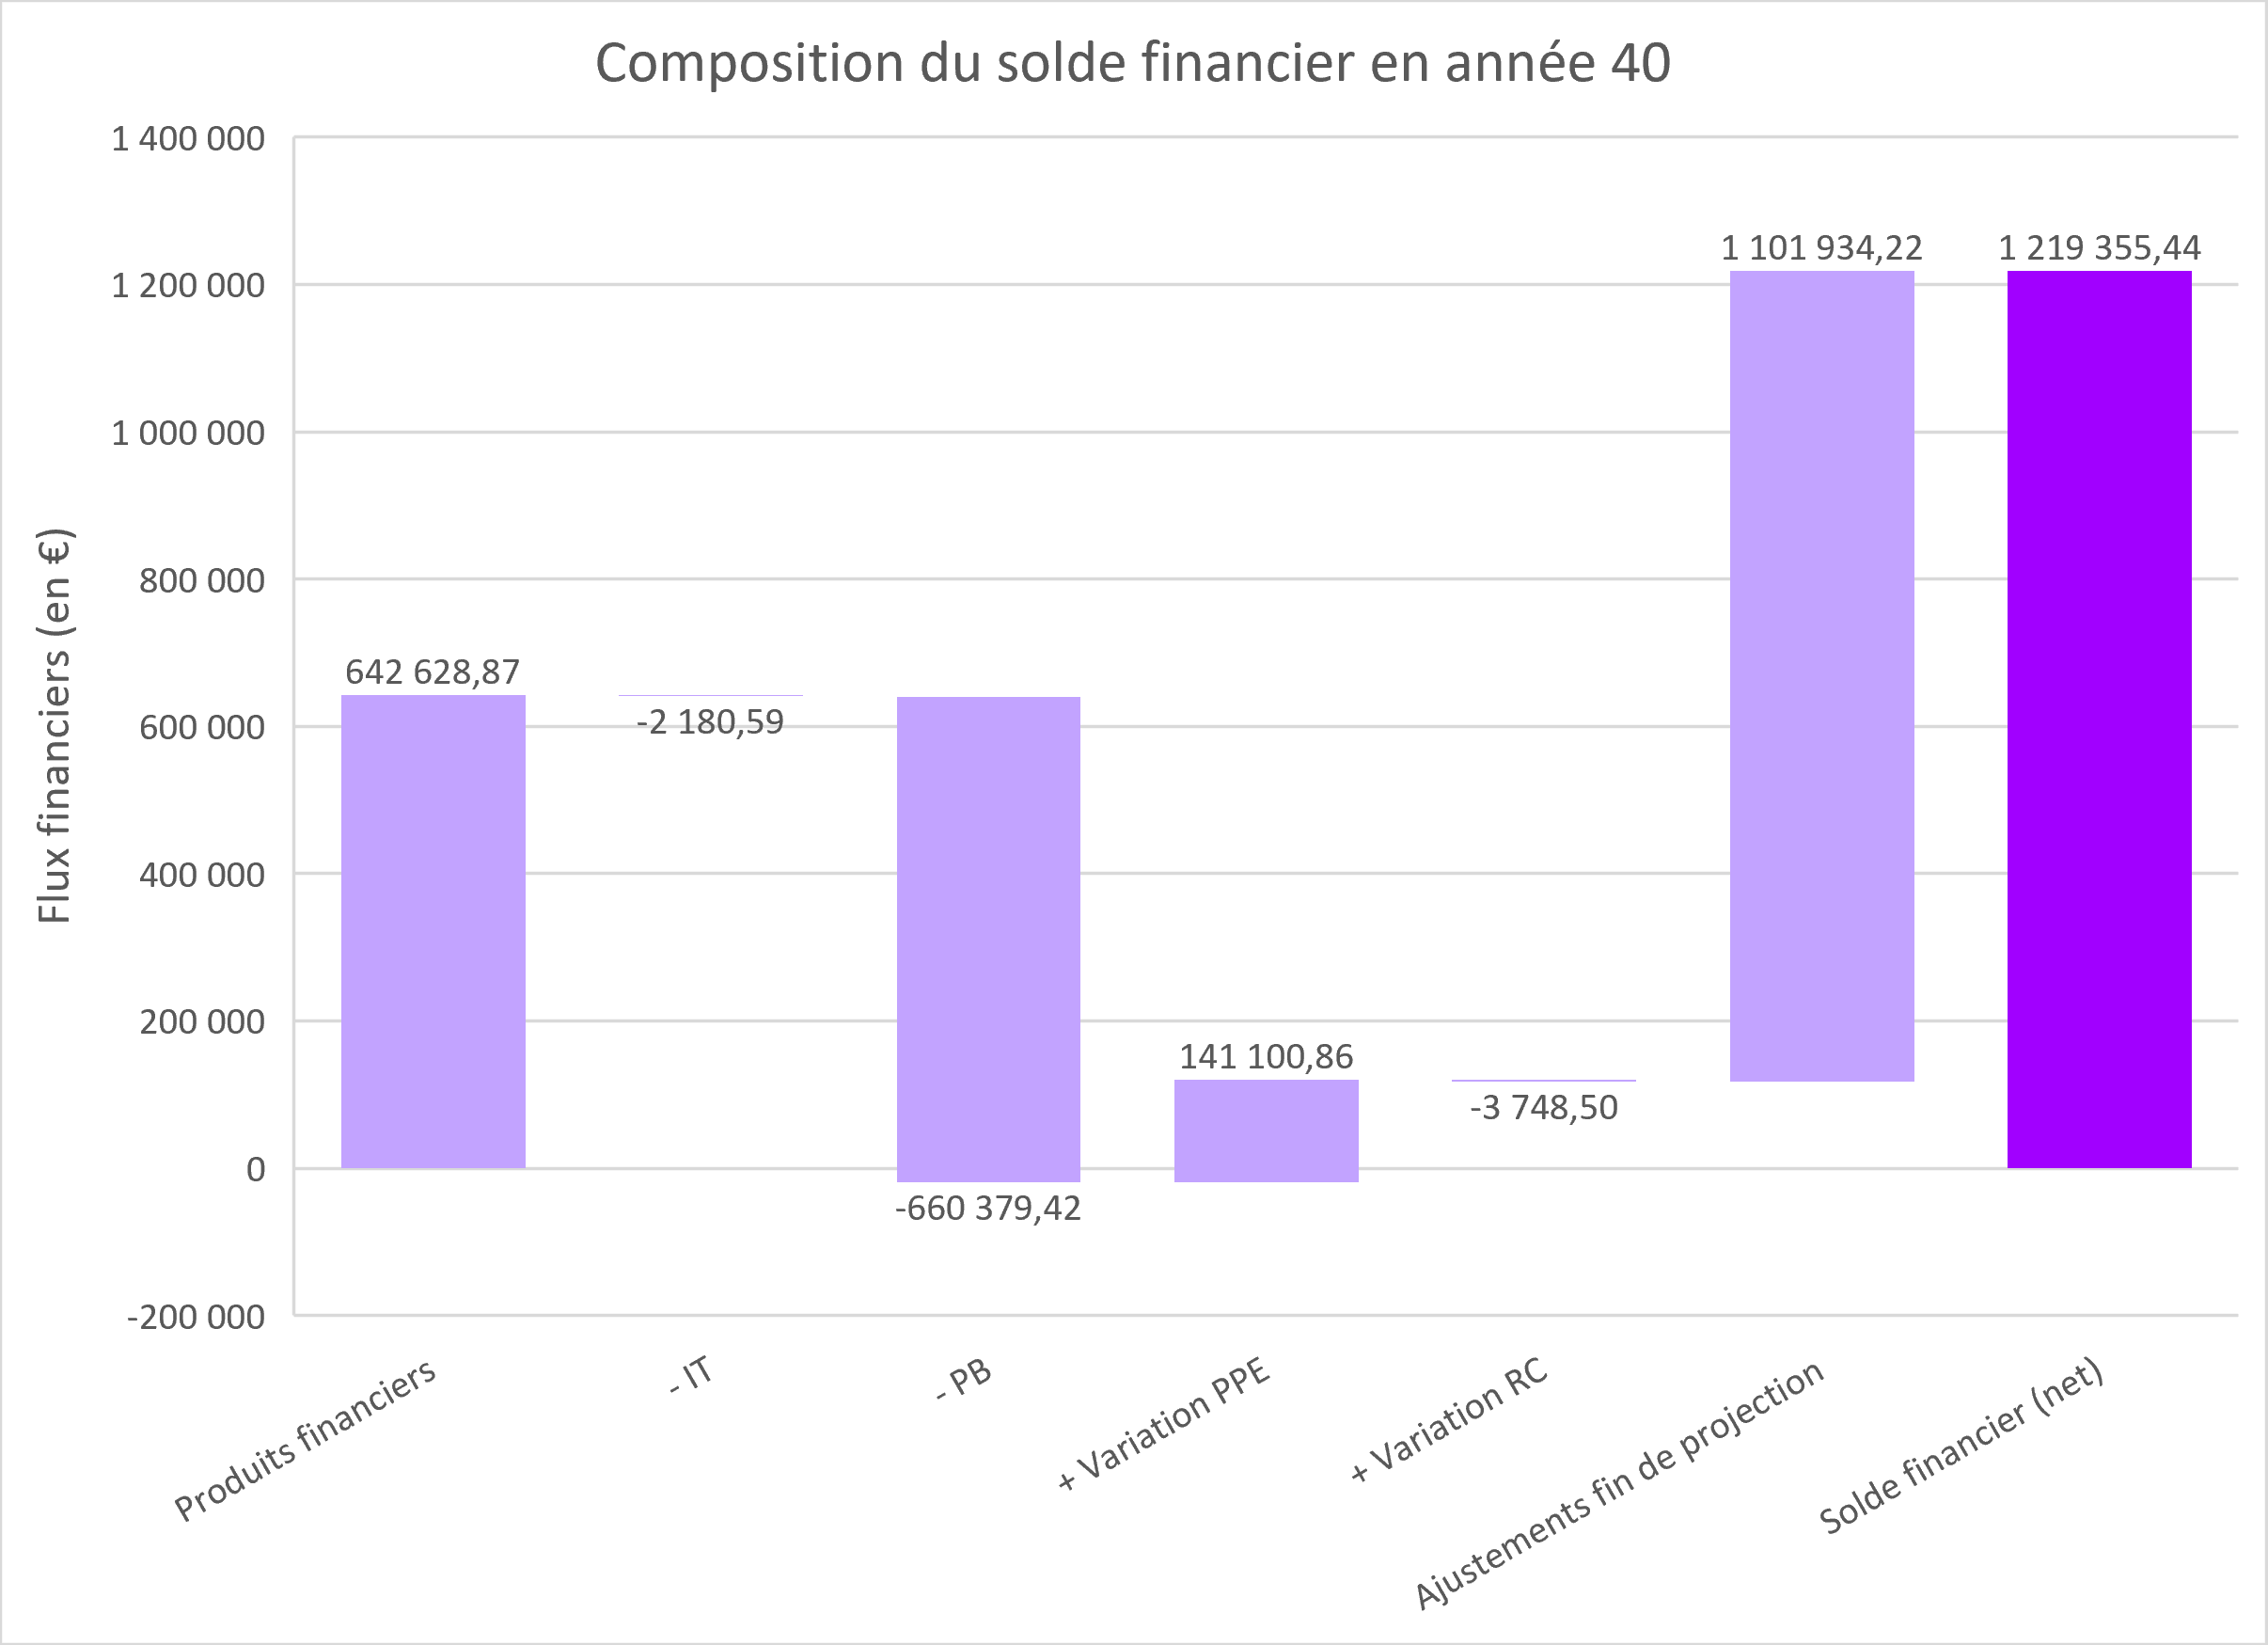
\includegraphics[width=0.65\textwidth]{images/compo_solde_financier_annee_40_mco.png}
    \caption{Composition du solde financier en année 40}
    \label{fig:compo_solde_financier_annee_40_mco}
\end{figure}

Les différents indicateurs analysés dans cette section racontent en réalité la même histoire sous plusieurs angles. Le portefeuille étant fermé (run-off, sans new business ni cotisation), la PM se réduit continûment. Cela tire mécaniquement à la baisse les rachats, les produits financiers et donc la marge financière. Par-dessus cette tendance structurelle, le mécanisme de pilotage de la PB introduit un décalage temporel : le taux servi reste en retrait du TRA tant que la PPE se constitue, ce qui alimente en retour des rachats conjoncturels plus élevés en début de projection, avant que la reprise progressive de la PPE n'inverse la tendance en fin d'horizon. La dernière année de projection doit enfin être interprétée avec prudence, c'est l'année de liquidation du portefeuille.

\section{Scénario témoin paramétré selon des avis d'experts}

Le calibrage par MCO présenté ci-dessus reflète la moyenne des dynamiques observées sur la période 2004-2025. Or cette période inclut une phase prolongée de taux bas, voire négatifs, qui n'est pas nécessairement représentative de l'environnement de taux que la BCE cherche à ancrer durablement à travers sa politique monétaire. Le second scénario témoin vise ainsi à corriger ce biais potentiel, en fixant à dire d'expert les paramètres jugés les plus sensibles à cet écueil, sur la base des objectifs et anticipations communiqués par la BCE, plutôt que de la seule moyenne historique.

\subsection{Calibrage des paramètres par avis d'experts}

Le tableau~\ref{tab:parametres_gse_experts} présente les paramètres du GSE calibrés selon une approche dite « à dire d'expert », en écho au tableau~\ref{tab:parametres_gse_MCO} qui reportait les estimations obtenues par la méthode des moindres carrés ordinaires (MCO) sur la période 2004-2025.
Cette calibration alternative vise à corriger les biais liés à la composition de l'échantillon historique et à ancrer certains paramètres sur des références macro-financières structurelles, telles que discutées ci-après pour chacune des variables concernées. Par souci de lisibilité, les valeurs modifiées par rapport à la calibration MCO sont indiquées en violet ; les autres sont conservées à l'identique.

\begin{table}[H]
\centering
\caption{Paramètres du GSE calibrés selon les objectifs dits d'experts}
\label{tab:parametres_gse_experts}
\begin{tabular}{llccc}
\hline
\textbf{Variable} & \textbf{Modèle} & $\hat{\kappa}$ \textit{ou} $\hat{\mu}$ & $\hat{\theta}$ & $\hat{\sigma}$ \\
\hline
Taux 10 ans (France)   & Vasicek & \textcolor[HTML]{A100FF}{0,1} & \textcolor[HTML]{A100FF}{0,03} & 0,00737 \\
Spread 1/10 ans   & Vasicek & 0,336 & 0,0107 & 0,006986 \\
Taux 30 ans (France)   & Vasicek & \textcolor[HTML]{A100FF}{0,05} & \textcolor[HTML]{A100FF}{0,035} & 0,00737 \\
Inflation (France)     & Ornstein-Uhlenbeck & \textcolor[HTML]{A100FF}{0,3} & \textcolor[HTML]{A100FF}{0,02} & 0,0123 \\
Actions (STOXX 600 NR) & GBM & 0,0776 & — & 0,139 \\
Immobilier (IEIF EZ)   & GBM & 0,0657 & — & 0,200 \\
\hline
\end{tabular}
\end{table}

Cette calibration s'écarte volontairement des estimations obtenues par moindres carrés ordinaires sur trois variables : le taux 10 ans, le taux 30 ans et l'inflation françaises. Le spread 1/10 ans, quant à lui, est conservé à l'identique.

Pour le taux 10 ans, le niveau de long terme est relevé de 2,02\,\% (MCO) à 3,0\,\% (expert), tout en réduisant la vitesse de retour de 0,146 à 0,1, soit une demi-vie portée de 4,7 à 6,9 ans. Cette double correction traduit l'hypothèse que l'échantillon 2004-2025 sous-estime le niveau d'équilibre de long terme en raison du poids disproportionné de la période de taux bas. Le niveau retenu de 3,0\,\% correspond à une évaluation du taux d'intérêt naturel nominal de la zone euro auquel s'ajoute la prime de risque souveraine française. C'est un niveau de long terme donc on espère que le taux 10 ans retrouvera ce niveau dans les années à venir. Le ralentissement corrélatif de $\kappa$ reflète l'idée qu'un changement de régime structurel, et non une simple fluctuation conjoncturelle autour de l'ancienne moyenne, met davantage de temps à se résorber.

Le taux 30 ans appelle une correction plus marquée encore, et constitue le cas le plus instructif de cette calibration. L'estimation MCO produit un résultat contre-intuitif : $\hat{\kappa}_{30\text{ans}}$ (0,176) est supérieur à $\hat{\kappa}_{10\text{ans}}$ (0,146), c'est-à-dire que le taux 30 ans reviendrait plus rapidement vers sa moyenne que le taux 10 ans. Ce résultat contredit la théorie de la structure par terme des taux d'intérêt, selon laquelle les maturités longues incorporent des anticipations lointaines et une prime de terme dont la dynamique est nécessairement plus lente que celle des maturités intermédiaires, un résultat également confirmé empiriquement par la littérature --- biblio --- sur la décomposition niveau/pente/courbure de la courbe des taux, où le facteur de niveau, qui domine les maturités longues, s'avère systématiquement le plus persistant. Le paramétrage impose donc $\kappa_{30\text{ans}} = 0{,}05 < \kappa_{10\text{ans}} = 0{,}1$, rétablissant l'ordre théoriquement attendu entre les deux maturités, et relève le niveau de long terme à 3,5\,\%, cohérent avec une prime de terme structurelle de 40 à 50 points de base au-dessus du 10 ans ??? .

Pour l'inflation, le niveau de long terme est abaissé de 2,23\,\% (MCO) à 2,0\,\% (expert), en s'appuyant sur la cible d'inflation à moyen terme explicitement fixée par la BCE depuis la revue stratégique de 2021 --- biblio ---. La moyenne MCO est en effet mécaniquement tirée vers le haut par le choc inflationniste de 2021-2023, un épisode considéré ici comme transitoire plutôt que représentatif d'un nouveau régime d'équilibre. $\kappa$ est relevé en parallèle de 0,198 à 0,3, soit une demi-vie ramenée de 3,5 à 2,3 ans, afin de traduire l'ancrage des anticipations d'inflation permis par la crédibilité de la banque centrale : un écart par rapport à la cible doit, par construction du mandat de la BCE, se résorber plus rapidement qu'une simple moyenne historique ne le suggère.

Un dernier point mérite d'être souligné : la cohérence croisée entre ces calibrations. Le spread 1/10 ans ayant été maintenu à l'identique ($\theta = 0{,}0107$), toute modification du niveau de long terme du taux 10 ans se répercute mécaniquement, via l'identité taux 1 an = taux 10 ans $-$ spread, sur le niveau implicite du taux à 1 an. Sous la calibration MCO, ce taux 1 an implicite s'établit à $2{,}02\,\% - 1{,}07\,\% = 0{,}95\,\%$, un niveau qui paraît aujourd'hui trop bas au regard du contexte de sortie des politiques monétaires ultra-accommodantes. Sous la calibration d'expert, il devient $3{,}0\,\% - 1{,}07\,\% = 1{,}93\,\%$, un niveau qui se situe dans la fourchette des estimations les plus récentes du taux d'intérêt naturel nominal de la zone euro (1,75\,\%-2,25\,\%). Cette cohérence, bien que non recherchée de façon délibérée au moment de fixer chaque paramètre isolément, valide a posteriori la calibration retenue. 

\subsection{Analyse des résultats du scénario paramétré selon les avis d'experts}

Sous ce paramètrage, le GSE génère 1\,000 trajectoires de marché ancrées sur des niveaux de long terme de taux plus élevés et des retours à la moyenne moins rapides. Les indicateurs ALM présentés ci-dessous reflètent les distributions de ces simulations sur un horizon de 40 ans.

\subsubsection{Le taux de rendement des actifs et le taux servi}

Le TRA moyen progresse de façon régulière et quasi monotone sur l'ensemble de l'horizon, passant d'environ 4,1\% à 5,4\%, sans rupture marquée de tendance (figure \ref{fig:tra_vs_tx_servi_experts}). Le taux servi moyen, lui, démarre nettement en retrait (3,1\%) et reste quasiment stable jusqu'à l'année 7-8, avant d'amorcer une hausse progressive qui s'accélère en fin de période, jusqu'à dépasser le TRA aux alentours de l'année 34 et finir au-dessus de lui (6,0\% contre 5,4\% en année 40).

\begin{figure}[H]
    \centering
    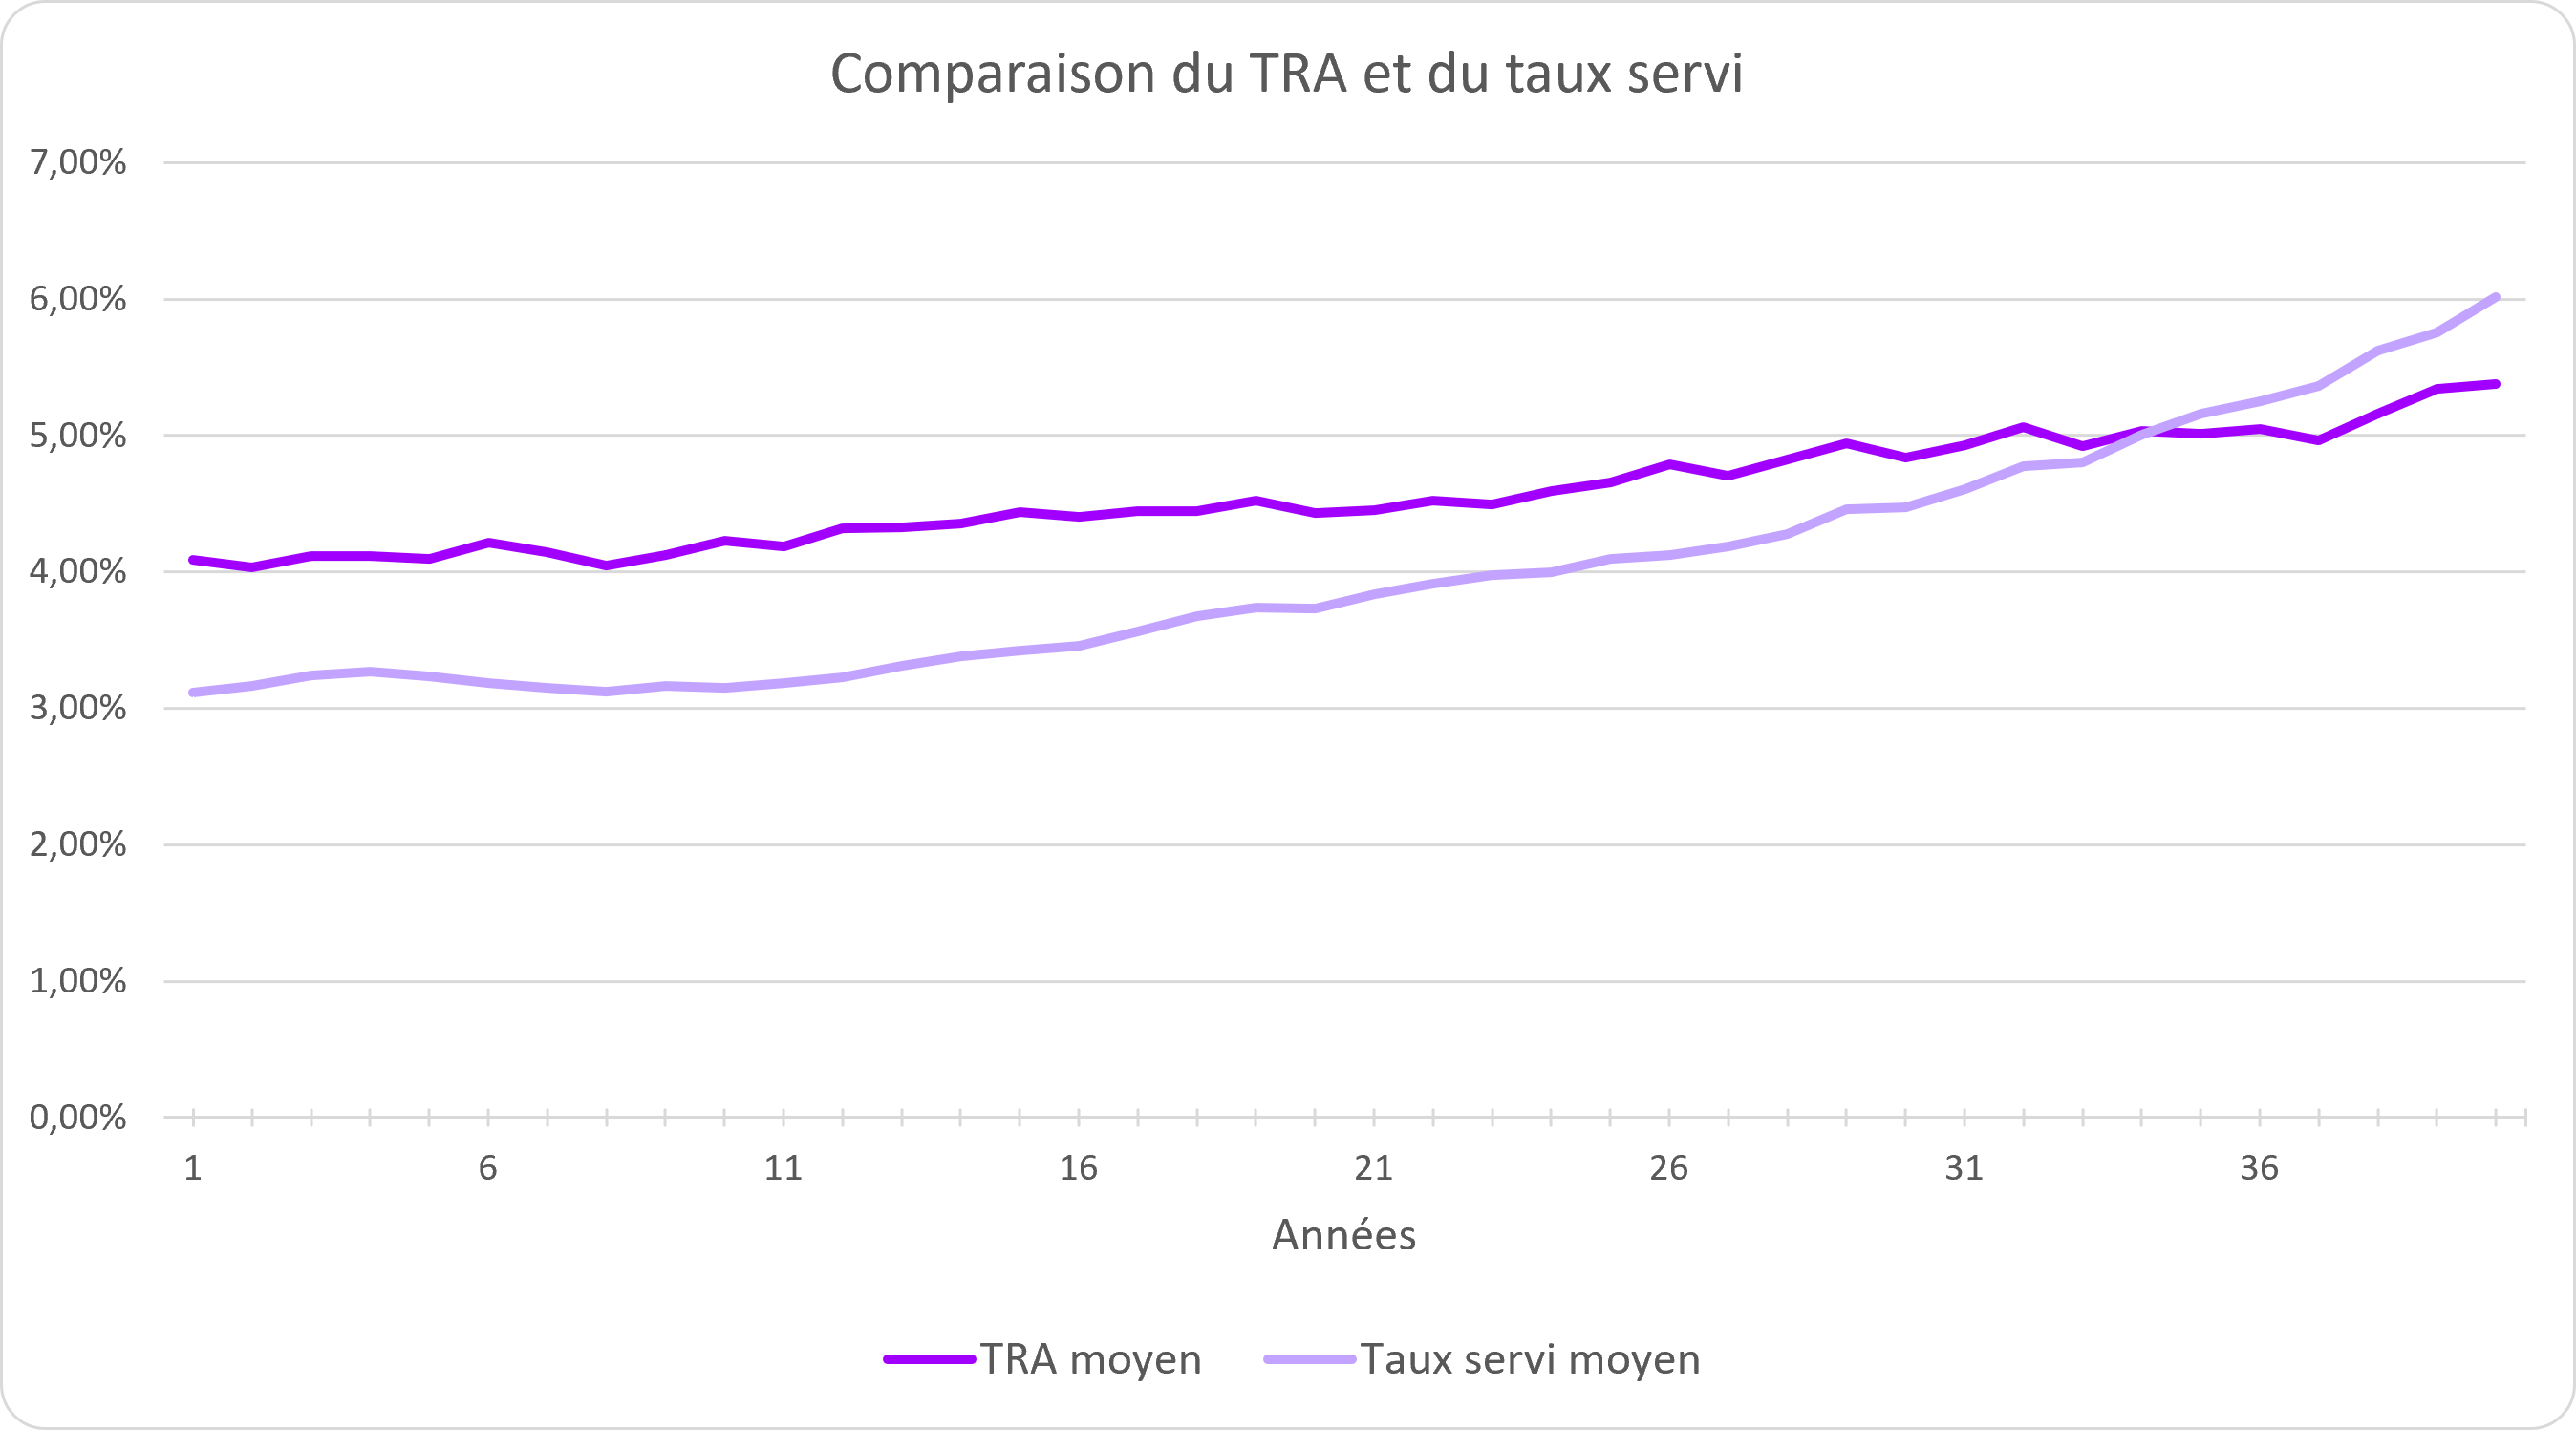
\includegraphics[width=0.65\textwidth]{images/tra_vs_tx_servi_experts.png}
    \caption{Comparaison entre le TRA et le taux servi sur 40 ans}
    \label{fig:tra_vs_tx_servi_experts}
\end{figure}

Cette dynamique se lit directement dans les flux de PPE (figure \ref{fig:variations_PPE_experts}). Les toutes premières années (1 à 4) affichent de légères reprises nettes, la PPE initiale servant à combler un écart ponctuel entre contractuel et cible. À partir de l'année 5 et jusqu'à l'année 17 environ, la tendance s'inverse : les dotations deviennent positives et significatives, avec un pic autour de l'année 12 ; cette phase correspond exactement au moment où le taux servi reste plat pendant que le TRA continue de grimper. L'écart croissant entre le contractuel (indexé sur le TRA) et la cible qui est, elle, lissée est capté et mis en réserve plutôt que distribué. Cela explique le plafonnement du taux servi sur cette période.

\begin{figure}[H]
    \centering
    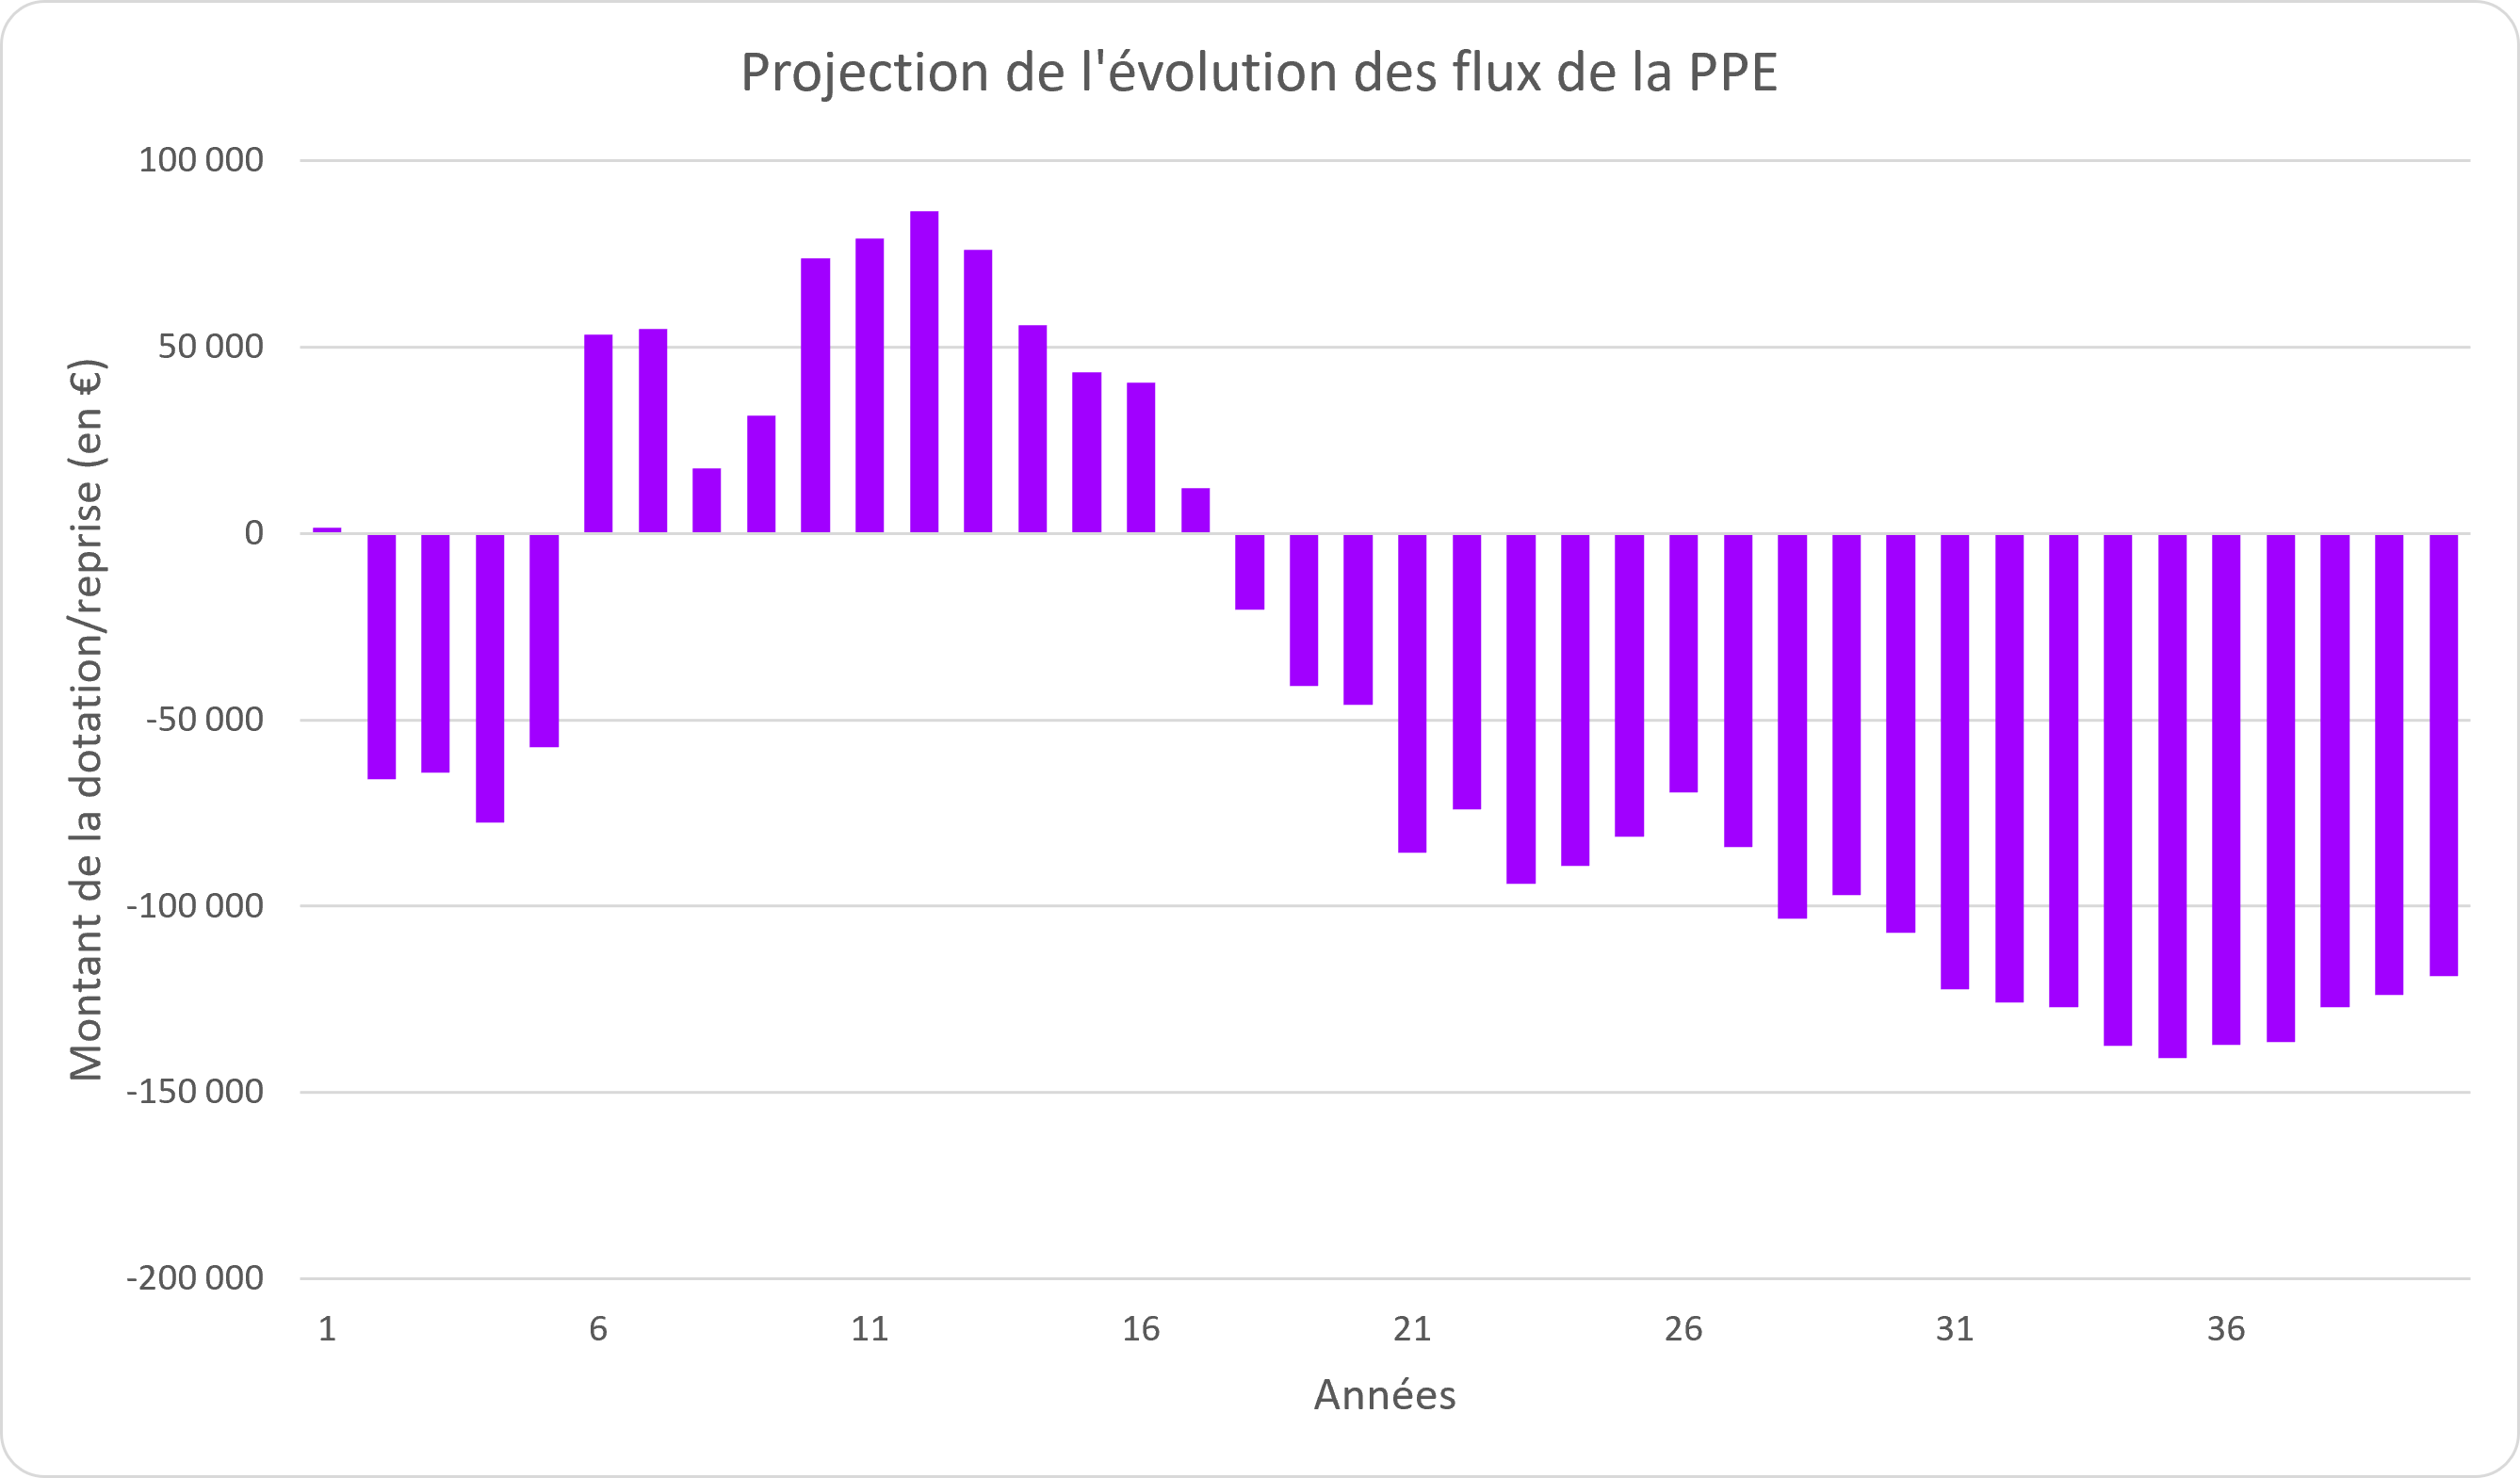
\includegraphics[width=0.65\textwidth]{images/variations_PPE_experts.png}
    \caption{Evolution des flux de la PPE sur 40 ans}
    \label{fig:variations_PPE_experts}
\end{figure}

À partir de l'année 18-19, le mouvement s'inverse durablement : les flux redeviennent négatifs et l'ampleur des reprises augmente progressivement jusqu'en fin de projection (au-delà de -100 000 € par an à partir de l'année 30). C'est cette reprise massive et prolongée de la PPE constituée pendant la phase de dotation qui alimente la hausse continue du taux servi observée en seconde moitié d'horizon, jusqu'à lui permettre de dépasser durablement le TRA. Le stock accumulé pendant les années de constitution devient ainsi suffisamment important pour financer une revalorisation supérieure au rendement courant des actifs sur une longue période, plutôt que de se limiter à un simple rattrapage ponctuel.



\subsubsection{Les rachats}

Les prestations de rachat décroissent progressivement jusqu'à devenir marginal en fin d'horizon. Cette décroissance de fond s'explique toujours par le run-off du portefeuille : sans new business ni cotisation, la PM se réduit chaque année, et le rachat structurel diminue mécaniquement avec elle.

On observe toutefois, sur la figure \ref{fig:prestations_rachat_euro_experts}, un plateau initial qui se stabilise aux alentours de 3 M€ sur les 8 premières années. Cela colle avec ce qu'on a observé sur le TRA et le taux servi de ce scénario : le taux servi reste en retrait par rapport au TRA pendant une phase de constitution de la PPE qui dure ici plus longtemps que d'habitude. Or le rachat conjoncturel réagit précisément à cet écart entre le taux servi et le taux de marché. En effet, tant que l'assureur sert moins que ce que le marché offre, les assurés sont incités à racheter davantage. Le plateau élevé des rachats reflète donc directement la durée de cette phase où le taux servi peine à suivre le TRA, avant que la baisse structurelle de la PM ne prenne le relais et n'entraîne la décroissance continue observée jusqu'en fin de projection.

\begin{figure}[H]
    \centering
    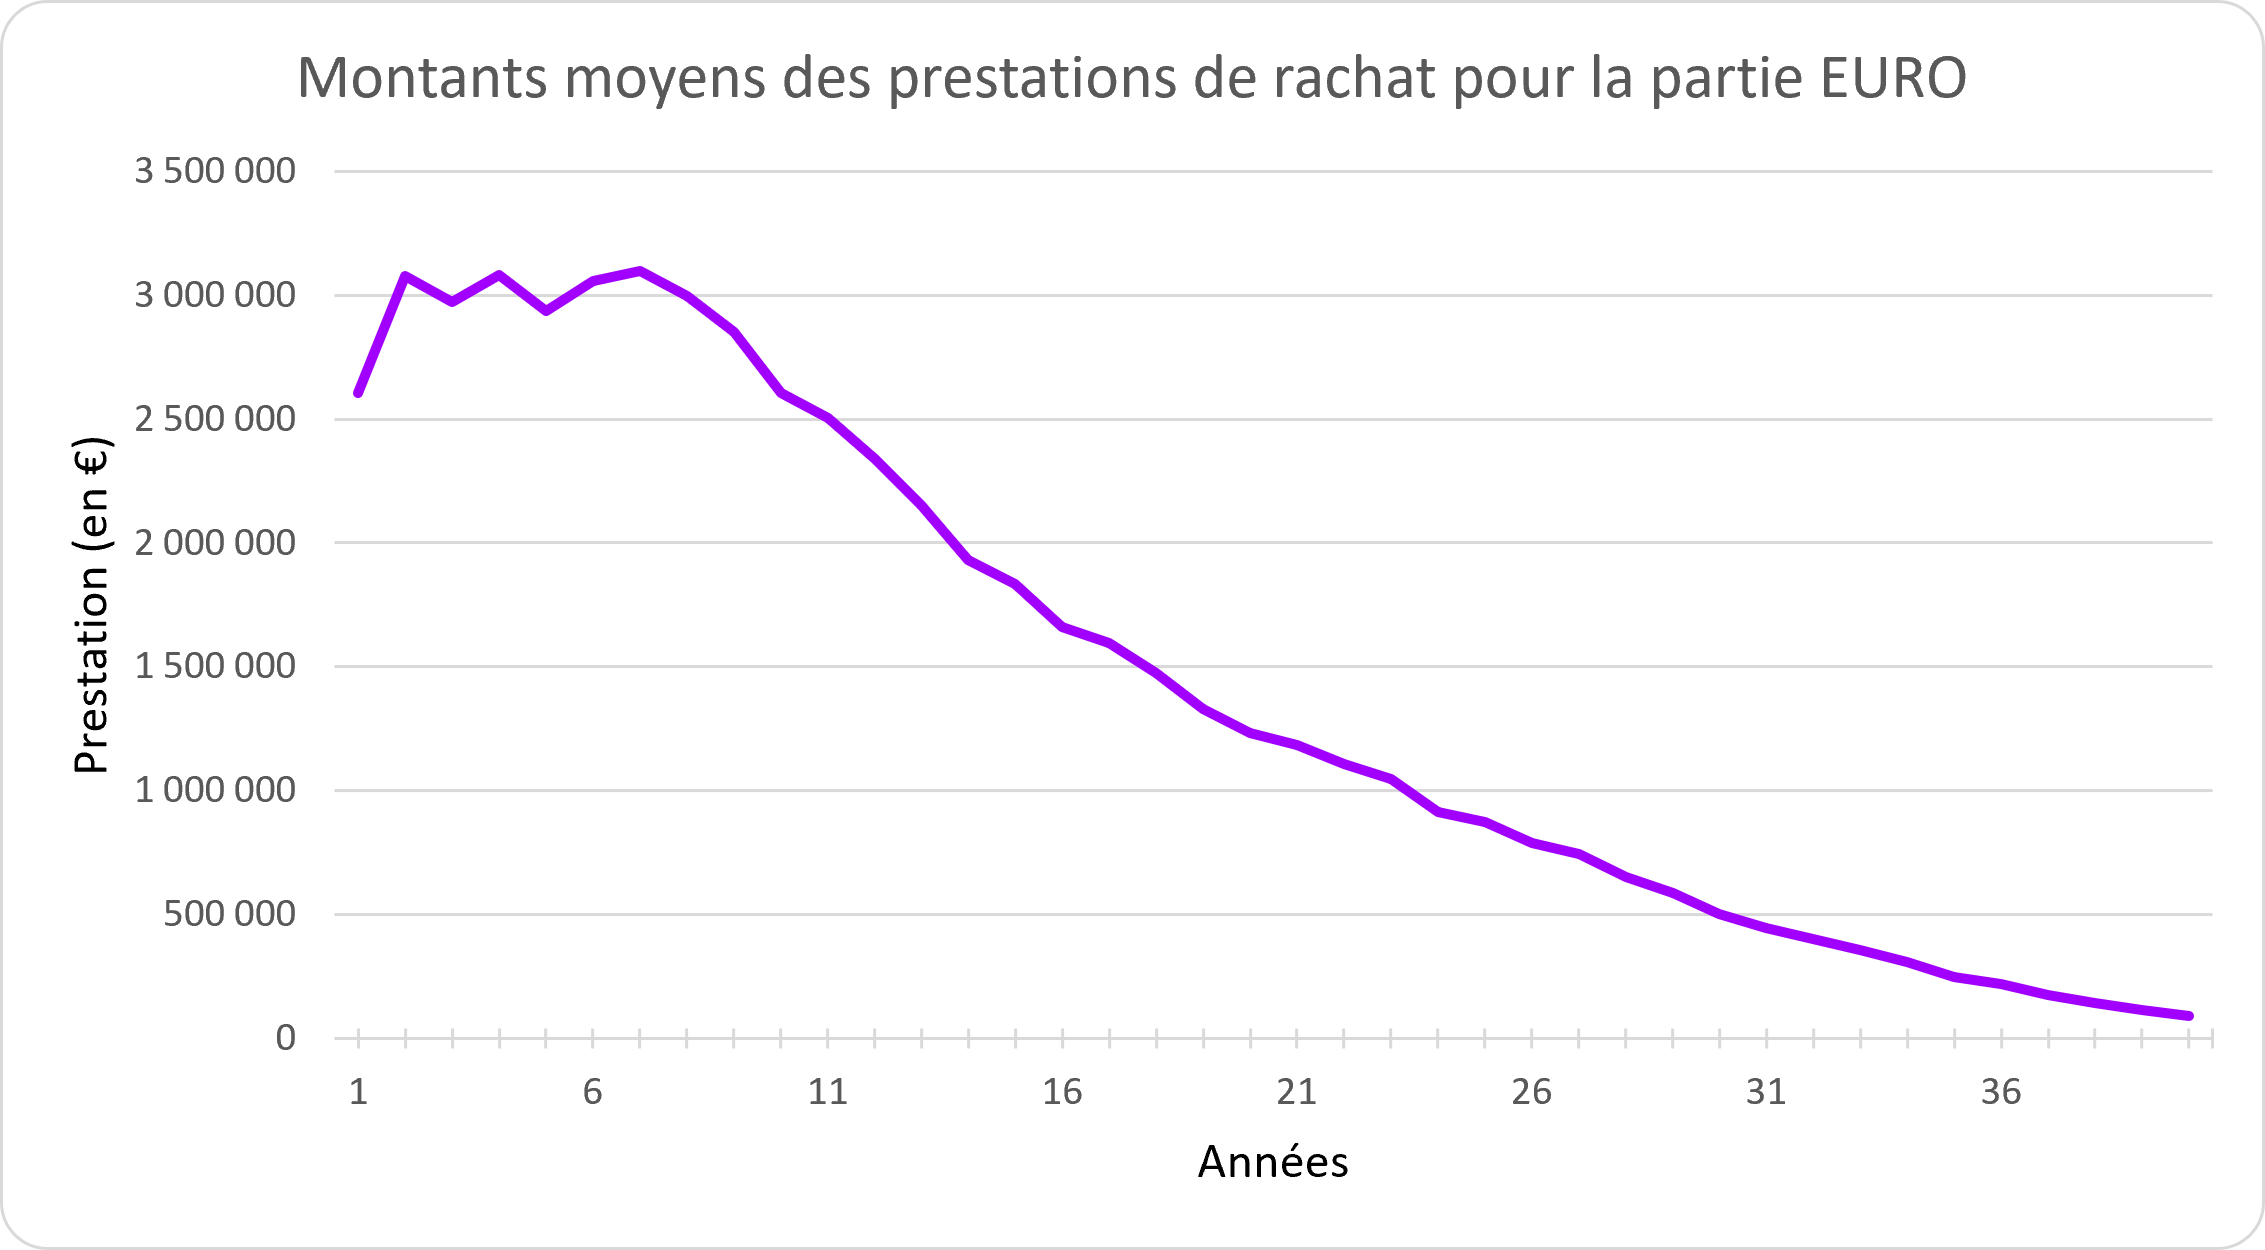
\includegraphics[width=0.65\textwidth]{images/prestations_rachat_euro_experts.png}
    \caption{Evolution des prestations de rachats sur 40 ans}
    \label{fig:prestations_rachat_euro_experts}
\end{figure}

\subsubsection{La marge financière}

Le solde financier décroît progressivement sur la quasi-totalité de l'horizon, porté par la baisse continue de la PM (portefeuille en run-off, sans new business ni cotisation) qui réduit d'année en année les produits financiers disponibles et donc la marge que l'assureur en retire. Le rebond brutal observé en toute dernière année (\ref{fig:solde_financier_experts}) n'est pas un signal de performance : il correspond aux ajustements de liquidation de fin de projection (reprise intégrale de la réserve de capitalisation, reconnaissance des plus-values latentes sur les actifs restants et d'une fraction de la PPE non distribuée), qui gonflent artificiellement le résultat de cette ultime année sans lien avec la rentabilité récurrente du contrat.

\begin{figure}[H]
    \centering
    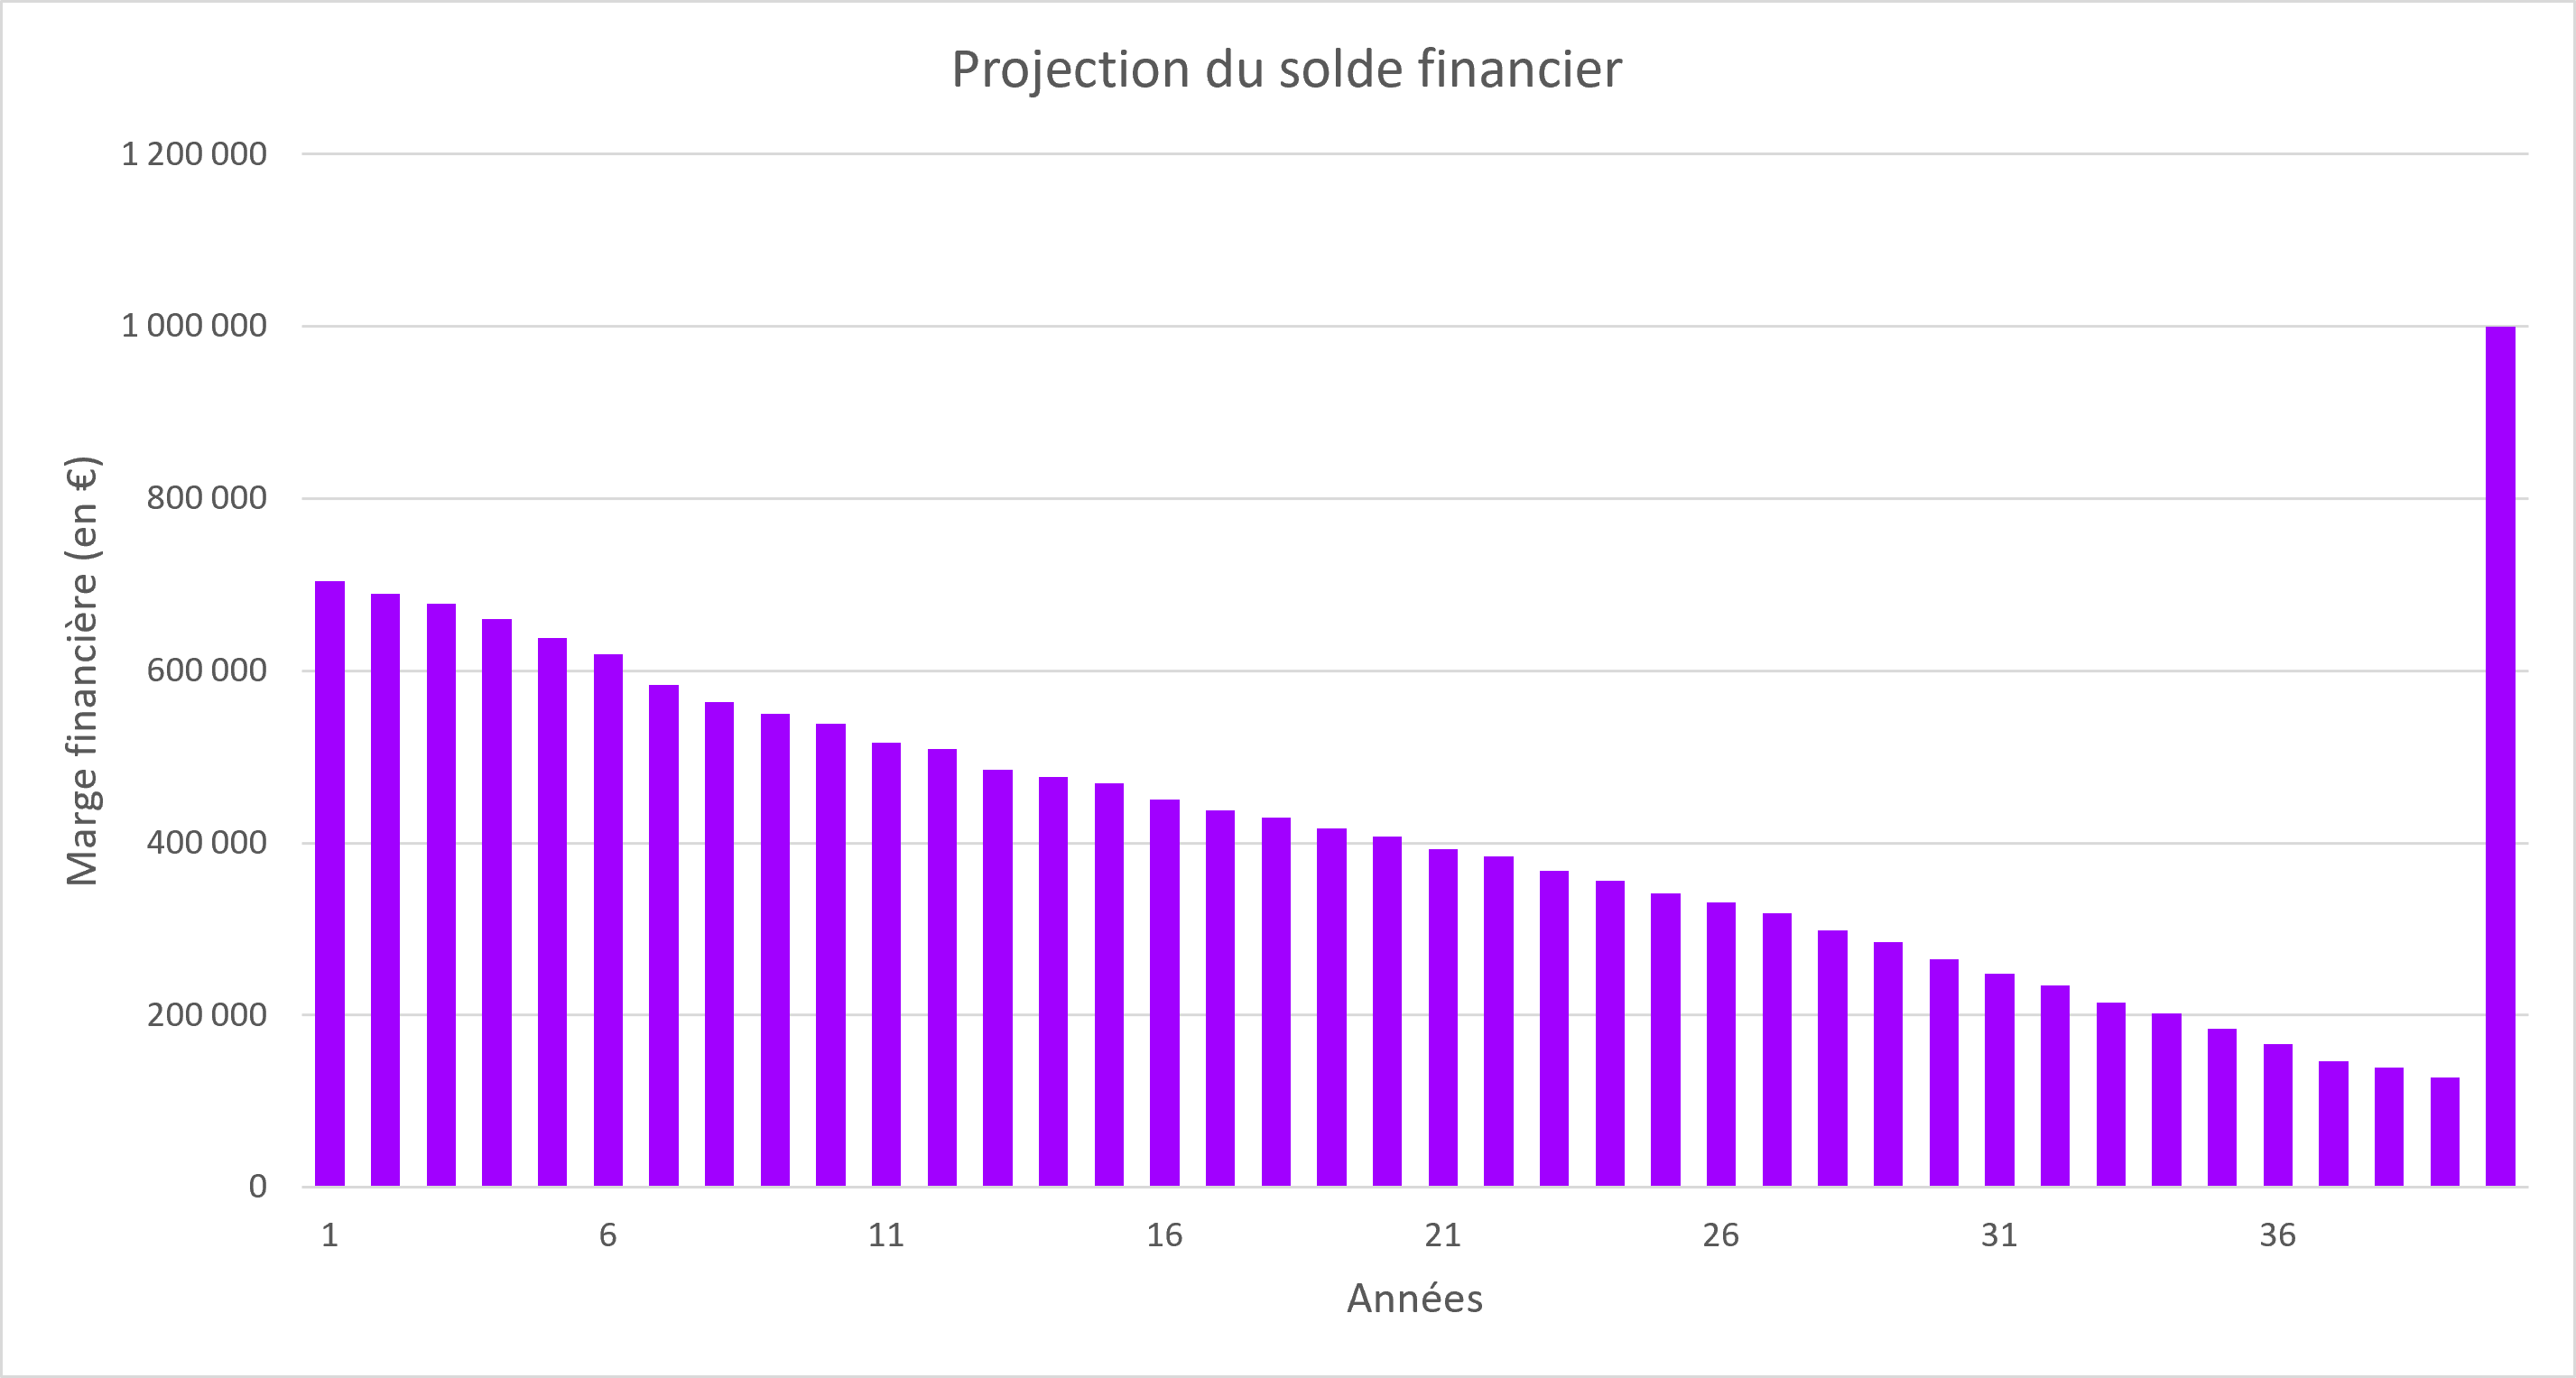
\includegraphics[width=0.65\textwidth]{images/solde_financier_experts.png}
    \caption{Evolution du solde financier sur 40 ans}
    \label{fig:solde_financier_experts}
\end{figure}


Au terme de cette analyse, les trois indicateurs racontent une cohérence interne : un TRA soutenu par un paramétrage de long terme élevé maintient un solde financier positif et stable en début de projection, mais cette même performance nourrit progressivement le taux servi via la PPE, ce qui finit par réduire la marge financière et par alimenter des rachats conjoncturels en phase de montée. La dynamique de run-off reste le facteur structurant dominant : les rachats font décroitre de manière continue la PM, ce qui réduit mécaniquement les produits financiers et donc la marge financière. 

\section{Comparaison des deux scénarios témoins et limites du modèle}
\label{sec:limites_runs_temoins}